\documentclass[12pt,a4paper]{book}
\usepackage[titletoc,toc,title]{appendix}
\usepackage{color}
\usepackage{colortbl}
\usepackage{graphicx}
\usepackage{algpseudocode}
\usepackage{graphicx}
% \usepackage{url}
\usepackage{verbatim}
%\usepackage{caption}
%\usepackage{subcaption}
%\usepackage{textcomp}
%\usepackage{fancyvrb}
\usepackage{graphicx}
\usepackage{amssymb}
\usepackage{epstopdf}
\usepackage{hyperref}
\usepackage{float}
\usepackage{adjustbox}
\usepackage{subfig}
\usepackage{placeins}
\usepackage{multirow}
%\usepackage[square]{natbib}
\usepackage[nottoc]{tocbibind}
\usepackage[pass]{geometry}

\definecolor{Gray}{gray}{0.8}
\definecolor{LightRed}{rgb}{0.99,0.9,0.9}

\newcommand\todo[1]{\textcolor{red}{#1}}

\begin{document}
\title{\small Thesis\\\huge Investigating Methods Of Annotating Lifelogs For Use In Search}

\author{Harry Scells\\harrisen.scells@connect.qut.edu.au\\\\\small Supervisor - Guido Zuccon\\\small g.zuccon@qut.edu.au\\}
\maketitle

\chapter*{Abstract}
The notion of `quantified self' in recent years is allowing people to more easily capture data about themselves. Lifelogging is an umbrella term which encompasses multiple personalised data gathering forms which primarily involves wearing a device that continuously records images of every day events via one minute snapshots. This process creates vast amounts of personalised data about the user, however there is currently no accepted way to search this data that can accurately retrieve moments of significance that a user may be interested in. Here, four annotation methodologies are investigated to discover their performance in a text-based image retrieval system. Manual and automatic annotations are compared to test if a annotations generated automatically can perform well on the same tasks as the manual annotations. Finally, each methodology is compared in terms of the cost to manually and automatically collect annotations.

The results of this research indicate that under ideal conditions, annotations which represent a query are the most effective in a retrieval task. This is compounded by the fact that on average they are the most cost effective annotation to collect of the four under investigation.

\chapter*{Acknowledgements}
Thank you to my friends and family for the massive amount of support and encouragement over the past year -- I could not have done this without it!

Most importantly I would like to thank my amazing supervisor Guido for the incredible opportunities and support he has provided me with -- and for motivating me to pursue honours in the first place. It has been a challenging but amazing year of learning, and I am very grateful.


\tableofcontents

\chapter{Introduction}

What if you had hundreds of thousands of images of your everyday activities collected through a lifelogging device and you wanted to search for meaningful events in this collection? Searching through large data sets of lifelogging images for insights about daily activities is a fast emerging area of research within the information retrieval domain~\cite{gurrin2014lifelogging}. A range of consumer products allow anyone to capture their daily activities and it is becoming increasingly popular~\cite{gurrin2014lifelogging}\cite{van2014future}\cite{askoxylakis2011log}. These devices are typically sold under the umbrella term of `lifelogging cameras'. Like precursors blogging and vlogging, lifelogging is the next step in this series of life event recording devices. Lifelogging not only benefits consumers who wish to document their lives, but also has applications for security and policing services where there is a need to search the images recorded through body cameras that are already being worn.

Preliminary research has provided an insight into how difficult searching lifelogging images is~\cite{scells2016qut}. The text-based search of images is most commonly referred to as text-based image retrieval (TBIR). This research considers text based search solutions for lifelogging search. The alternative, content-based image retrieval (CBIR) does away with textual features and relies on the visual features of an image; for example colour, shape or texture, but generally assumes querying is through an example query image. In a study by Hartvedt~\cite{hartvedt2010using}, it was found that the benefit of TBIR over CIBR is that is supports image retrieval based on high-level textual semantic concepts. This claim is supported by Shao et.al~\cite{medical2004shao} who notes that TBIR exploits semantic information in the text associated with images. CBIR is not applicable as images are searched with textual queries only and, as stated before, CBIR assumes querying occurs through example images. TBIR is the predominant approach for image retrieval and most commercial search engines rely on this scheme~\cite{escalante2007towards}. TBIR intuitively relies heavily on quality annotations; if annotations have grammatical and spelling errors or do not correctly describe the content of the image (no semantic context) then the retrieval effectiveness is degraded. The requirements of a `good' textual document in, for example, web search, also applies to annotations of images.

Currently, no machine learning approach can consistently and reliably generate concepts (or annotations) from lifelog images due to the difference between the training data and the data contained in lifelogs. There are multiple methods of annotating images automatically, however this research is primarily focused on investigating the performance of manual annotations. A number of annotation methodologies are tested to find the most appropriate type of annotation for text based image retrieval of lifelog images.

Collecting annotations is important, but another important challenge is to determine which annotation methodology is the best for text-based image retrieval. Evaluation of images generally relies on gold standard annotations, none of which exist for lifelog images. The problem becomes clear - the standard ways of evaluation are not applicable to lifelog annotations unless a reference exists. A framework involving TREC-style\footnote{\url{http://trec.nist.gov/}} runs is used for evaluating arbitrary types of annotations associated with lifelog images. The quality of the annotations is evaluated by means of using annotations to inform the image representation in a TBIR system for lifelog search. The pipeline for evaluating lifelog images and their annotations and the data produced is an important and meaningful contribution of the thesis. 

Due to the sheer volume of annotations required to collect in the short time frame allowed by this thesis project and by the limited resources available for manual annotation, automatic image captioning is also investigated as part of this research. In this thesis, an image captioning system is trained on the manually collected annotations in order to annotate the entire collection of lifelog images. The collection of image is obtained form the the NTCIR-12 lifelog semantic access task (LSAT). The NTCIR-12 LSAT is a pilot task which has research teams retrieve and rank lifelog images using textual queries. The results from this research can be compared with the results from the NTCIR-12 LSAT to determine if the methods for image annotations investigated here improve over the performance of previous attempts.

\section{Aims and Objectives}

Four annotation methodologies are chosen as a basis for this research. Each methodology involves the collection of annotations through some interface and evaluation. The aim of the project is to determine the best methodology for annotating lifelog images. The four methodologies under investigation are: 

\begin{enumerate}
    \item Tags --- Sets of keywords that describe objects and semantics of an image. Tags are chosen from a user-defined, non persistent vocabulary. These are similar to what one would expect to see on Flickr and other similar sites.
    \item Textual Descriptions --- Descriptive long-form annotations that contain semantic meaning. These are similar to the contents of documents such as web pages or news papers.
    \item Relevance Assessments --- Images are scored on a 0-10 scale by how relevant the image relates to a given concept. These are more purposely obtained, similar to editorial efforts by commercial search engine companies.
    \item Reverse Queries --- Queries are formulated for a given search result listing. Annotators are asked to provide a query that they think would result in the image being returned by a typical search engine. These are more akin to what one would expect to see in query logs.
\end{enumerate}

To collect these annotations, interfaces are developed to facilitate the entering and recording of the annotations. Once a suitable number of annotations have been collected, each methodology is evaluated. The evaluation strategies available are explored as part of this research.

This research also aims to produce two meaningful contributions to the lifelog research community. Recent results from the NTCIR-12 conference indicate lifelog search engines which incorporate image processing in some way perform much better than simply using annotations alone~\cite{safadilig2016ligmrim}. A new higher quality collection of annotations for lifelog images as well as training data for image classification systems is expected to boost the performance for everyone researching lifelog search engines: the annotations are released to the research community. This directs future efforts for collecting and evaluating annotations and can act as a comparison for future lifelog annotations.

Finally, automatic image captioning is investigated. Here, a state-of-the-art image captioning pipeline generates captions for images using the manually collected annotations as training data. The end result is a fully annotated collection of lifelog images. Previous attempts at using textual descriptions as annotations~\cite{scells2016qut} resulted in poor, but optimistic results. 

Of the four annotation methodologies selected for investigation, a recommendation is made on the most effective of these and the results of the automatically generated captions are compared to the results of the manually collected annotations. 

\section{Research Gaps}

Two gaps are identified in the research through reviewing the literature. Annotation of lifelog images and their evaluation is not a standard process. Through preliminary research, a number of techniques have been investigated which are applicable to annotating images. A number of textual summarisation evaluation methods have also been considered, however none of these are capable of evaluation without a ground truth or gold standard. According to an examination of evaluation in information retrieval~\cite[p. 24]{sanderson2010test}, there has been very little work done to evaluate how good a test collection is. Furthermore, finding all relevant documents to build topics is still the accepted approach for creating a test collection~\cite{cooper1973selecting}.

It is currently unknown which annotation methodology most suits a lifelog images for a given TBIR system. This also implies that given a collection of lifelog images, it is unknown which form of annotation methodology for the images results in the best performance. Annotations (in general~\cite{snow2008cheap}) are very expensive to collect in both time and financially, thus determining the most appropriate methodology of annotation prior to collecting annotations is highly important.

\section{Research Questions}

This thesis aims to answer the following research questions:

\textbf{Research Question 1:} How can annotations for a collection of lifelog images be evaluated?

It is important that the annotations of images are accurate and of a high quality. Low quality annotations lead to poor evaluation results. Evaluation is performed without using a gold standard annotation, since this does not exist. In this way, this research uses the ad-hoc TREC-style approach used in the NTCIR-12 lifelog semantic access task. This evaluation methodology is also referred to as extrinsic evaluation, whereby annotations are evaluated by determining the performance of a larger system as a whole with respect to each annotation methodology.

\textbf{Research Question 2:} What methods could be used to annotate lifelog images and what is the retrieval effectiveness of annotations collected with these methods?
% What are the possible ways lifelog images can be annotated and what is their retrieval effectiveness?

There are many state of the art solutions for automatically summarising the contents of images~\cite{karpathy2015deep}\cite{jia2014caffe}\cite{pan2004gcap}, however this project involves measuring the effectiveness of manual annotations. This is due to the fact that training data specifically for lifelog images does not exit. This makes it challenging to train a model that can identify the contents of a lifelog image. In manually annotating images, a well formed collection of annotated lifelog images is produced and machine learning and computer vision algorithms can exploit this.

\textbf{Research Question 3:} RQ3: How do annotations generated by current state-of-the-art automatic image captioning techniques compare to the effectiveness of manual annotations?

The captions generated by machine learning are able to be evaluated in the same way the manual annotations are; the format of the annotations will not differ. The effectiveness of these automatic annotations provides a good comparison to the manually collected annotations and offers insight into how good the manual annotations are as training examples. Unlike the manual annotations, the automatically generated annotations are for the entire collection of lifelog images. 
\chapter{Background}

This chapter presents a background on the current state of searching lifelog images. This is done through a review of the literature and findings from the NTCIR-12 lifelog semantic access task. 

% ---------------------------------
%  BEGIN LIT REVIEW
% ---------------------------------
\subsection{Representing the Data}
One way of viewing lifelogging is the process of creating a surrogate memory for a person. Organising and presenting are the key challenges for lifelog search engines. Gurrin et al.~\cite{gurrin2014lifelogging} proposes that it is possible to segment the raw, unprocessed lifelog data into meaningful units, or events; which he defines as: "a temporally related sequence of lifelog data over a period of time with a defined beginning and end". In order to perform information retrieval, the events need to be annotated with meaningful semantics. Annotations can either be manually created by humans, or generated through machine learning algorithms. These annotations must also be evaluated for effectiveness, as poor annotations will lead to poor performance when performing retrieval on the images.

There are five aspects of human memory access, as proposed by Gurrin et al.~\cite{gurrin2014lifelogging}:
\begin{enumerate}
    \item Recollecting: Concerned with re-living and accessing past experiences of episodic memories.
    \item Reminiscing: A form of recollecting, concerned with reliving past experiences for emotional or sentimental reasons.
    \item Retrieving: A more specific form of recollecting  in which specific information needs are to be retrieved such as an address, a document, a location, or any atomic piece of information.
    \item Reflecting: A form of quantified-self analysis, performed in order to discover knowledge and insights that may not be immediately obvious.
    \item Remembering: Concerned with prospective memory more than episodic memory. A form of planning for future activities or to act as a reminder or prompt for tasks that a person would like to do.
\end{enumerate}
Gurrin et al.~\cite{gurrin2014lifelogging} argues that an information retrieval system targeted at lifelogging should focus on the Five R's as information needs for the user.

In the context of searching images on the web,  L. Vuurpij, et al.~\cite{vuurpij2002vind} states that image retrieval systems are restricted to the domain they cover and require a lot of domain knowledge in order to fulfil the information needs of a user. Furthermore, L. Vuurpij, et al.~\cite{vuurpij2002vind} notes that there has been a shift from computer vision and pattern recognition to psychology and cognitive science in the domain of image retrieval, where models like the Five R's~\cite{gurrin2014lifelogging}, are becoming more prevalent. 

\subsection{Annotating Lifelog Images}
The current state of the art models for image retrieval use tag-based or textual description annotations \cite{ali2010semantically}. This is typically due to the fact that retrieval models can use this text as a bag of words, or use the text to attribute some form of semantic meaning.

\subsection{Evaluating Annotations}
Without high quality annotations, semantic search would not work, since semantic search exploits the meaning and context of a sentence rather than the keywords in it \cite{ali2010semantically}. The semantic and contextual data associated with images is important for an effective retrieval model that uses textual features rather than pixel data in images. This textual data can either be generated using machine learning algorithms, as demonstrated by A. Karpathy et al.~\cite{karpathy2015deep} and  I. Sutskeve et al.~\cite{sutskever2011generating}, or generated manually by humans. The machine learning algorithms do however start from test data, typically of a specific domain or a range of domains, which they learn from. It is important to note that this can have undesirable consequences when trying to apply a model which has been trained on one domain to one which it has no knowledge of. In both situations, it is essential that the annotations themselves are evaluated such that they describe the image with enough detail and are convincing to humans, since queries will be formulated by humans. Three widely used models for this exist: BLEU \cite{papineni2002bleu} which is precision based, ROUGE (Recall-Oriented Understudy for Gisting Evaluation) \cite{lin2004rouge} which is recall based, and METEOR \cite{elliott2013image}, used for judging the overall quality of annotations.

All of the metrics above were initially proposed with respect to the evaluation of automatic summarisation and natural language processing. Furthermore, they all use a reference annotation in order to score annotations. ROUGE compares the number of overlapping n-grams, word sequences, and word pairs of annotations with ideal annotations created by humans \cite{lin2004rouge}. BLEU counts the maximum number of times a word appears in any reference annotation, followed by "clipping" the total count of each candidate word by its maximum reference count, adding these "clips" up, and dividing by the total unclipped number of candidate words in the annotation \cite{papineni2002bleu}. The notion of "clipping" in BLEU is a variation of precision whereby words are only accepted for the maximum number of times they appear the reference text, for instance if a word appears in an annotation five times but is in the reference annotation twice, the "clipped" value would be 2/5. Finally, METEOR generally operates by unigram matching (bag of words) between a reference annotation, typically created by a machine, and a human produced annotation. Both METEOR and ROUGE take multiple approaches to comparing annotations, for reference, ROUGE:
\begin{enumerate}
    \item ROUGE-N N-gram Co-occurence Statistics
    \item ROUGE-L Longest Common Subsequence
    \item ROUGE-W Weighted Longest Common Subsequence
    \item ROUGE-S Skip-Bigram Co-Occurence Statistics
    \item ROUGE-SU Skip-Bigram Co-Occurence Statistics with Unigram\\ Counting Unit
\end{enumerate}
The unigrams matched in METEOR can be based on surface forms, stemmed forms, and meanings, with the option to be extended \cite{elliott2013image}.

R. Vedantam et al.~\cite{vedantam2015cider} argue through the results of their experimentation, however, that there exists a more effective model for evaluation which is rooted in human consensus. Their method, CIDEr (Concensus-based Image Description Evaluation) is a model which outperforms all other models of evaluating descriptive annotations of images. CIDEr performs so well due to high correlation with human judgement and consensus. According to R. Vedantam et al.~\cite{vedantam2015cider}, the CIDEr metric inherently captures sentence similarity, the notions of grammatically, salience, importance (precision), and accuracy (recall). CIDEr appears to improve upon the other three models and takes into account the weaknesses the other models may have, however it still relies on reference annotations.

The evaluation methods above rely on the availability of a ground truth or reference annotation that can be used to compare with the automatically generated annotation. This approach, however, is ill-suited to generating annotations for lifelog images as it is unclear what these annotations should ``look like'', because it is unknown what makes an annotation of a lifelog image ``good''. A better suited alternative for this problem is to embed the evaluation of different annotation methods within a task and thus evaluate the  methods with respect to the effectiveness the different methods induce on the task. Specifically, in this research project, the aim is to embed the evaluation of lifelog annotation within a search task. Thus the effectiveness of a system would be evaluated with respect to the search task. None of the system properties would vary apart from the method that is used to annotate images.This evaluation methodology is akin to, for example, previous work that has examined the effectiveness and quality of different topic modelling techniques and semantic models via evaluating the effect they have on search engine result effectiveness~\cite{wei2006lda,zuccon2015integrating,karimzadehgan2010estimation,yi2009comparative}.

\subsection{Types of Annotations}
As suggested by R. Yan et al.~\cite{yan2008learning}, the most common image annotation approaches can be categorised into two types. The first is \textit{tagging}, where annotators choose a set of keywords from a vocabulary for each image. The second most common approach is described as \textit{browsing}, where a group of images are judged against the relevance of a predefined keyword. There are, however, less commonly used annotation approaches, for example, \textit{descriptive natural language annotations} which are generated in a model by A. Karpathy et al.~\cite{karpathy2015deep}. This model outperforms the previous work done in this area of research for both image retrieval and image annotation on the Flickr8K, Flickr300K and MSCOCO. B. Hu et al.~\cite{hu2003ontology} clarifies why high quality textual descriptions generally perform better than systems that employ keyword or tag based annotation models, in that these models suffer from several limitations:
\begin{enumerate}
    \item A keyword in a document does not necessarily mean that the document is relevant
    \item A relevant document may not contain the explicit word
    \item Synonyms of the query keywords lower the recall rate (ratio of retrieved images which are relevant to the total number of relevant images, see Appendix A for details)
    \item Homonyms of the query keywords lower the precision rate  (ratio of relevant images that are successfully retrieved to the total number of relevant and irrelevant images retrieved) see Appendix A for details)
    \item Semantic relations such as hyponymy, meronymy, antonymy are not exploited
\end{enumerate}

Recent work in the consumer health search domain by Zuccon et al.~\cite{quteprints82599} and Stanton et al.~\cite{stanton2014circumlocution} focused on generating queries from images. The aim of their research was to understand how the general public would search for information if they had a medical condition as that in the image presented to them. This new methodology used by these previous works could be adapted to the context of gathering annotations for lifelogging, thus leading to an \textit{annotation by querying} method. This method would consist of showing annotators an image from a lifelogger and ask them to provide the queries they would issue to a (standard) search engine to attempt to retrieve the image itself.

\subsection{Searching for Lifelog Images}
Lifelog information retrieval systems typically have very poor performance due to there not being any formal models made specifically for the field, as reported by Gurrin et al.~\cite{gurrin2014lifelogging}. Until very recently, there have been no large, distributable test collections such as the TREC collection for text \cite{gurrin2014lifelogging}. The NTCIR collection is a set of tagged lifelog images which have been collected by researchers who wore a lifelogging camera for a short amount of time \cite{gurrin2016ntcir}. The tags were automatically generated by using a pre-trained image tagging algorithm.

While there is limited applied methodology to retrieval models in lifelogging, there has been much discussion about what the models should try and solve. Both H.  W.  Bristow et al.~\cite{bristow2004defining} and A. R. Doherty et al.~\cite{doherty2010automatically} corroborate that detecting and interpreting the implicit semantics and context of lifelogging data from heterogeneous sources would be advantageous in explaining the Who?, What?, Where? and When? questions which occur in every day events. It was also noted that these questions are common among image searchers and that they are not capable of being answered by normal indexing like that in traditional search engines \cite{ali2010semantically}.

While there has been some research into tagging and annotating images, there has not been as much work in developing a model for searching these images within the context of lifelogging \cite{gurrin2014lifelogging}. Typical image search engines for web pages treat the surrounding text, captions, alternate text and HTML titles \cite{frankel1996webseer} as a bag of words for retrieval. The success of these search engines rely on a sufficient amount of surrounding text, something which is not provided by current automatic image annotation models for lifelogging. The longer and more detailed the text is within the context of the image, the better the performance of the search engine. This is perhaps why other research has involved novel search techniques \cite{vuurpij2002vind}, since the current models for generating captions of images are not yet detailed or accurate enough for current textual information retrieval models to work.

Generally, image based retrieval methods can be classified into two categories: text-based image retrieval (TBIR) and content-based image retrieval (CBIR). A CBIR system utilises image features such as grid colour movements, edge direction histogram, Gabor textual features, and Local binary pattern histograms. as described in work by Wu et al.\cite{wu2009distance}. These features (colour, texture, shape, SIFT keypoints) become a query to the search engine which match visually similar images. CBIR systems, although extensively studied for over a decade, are still limited in comparison to TBIR systems. Zue et al.\cite{zhu2010image} provide three points for why this is:
\begin{enumerate}
    \item The semantic gap that exists between low-level visual features and high-level semantic concepts
    \item The low efficiency due to high dimensionality of feature vectors
    \item The query form is unnatural for image searching (appropriate example images may be absent)
\end{enumerate}
The efficiency of TBIR can be explained when one considers that it can be formulated as a document retrieval problem and can be implemented using the inverted index technique. The downside to TBIR is that is highly expensive: experimental evidence by Wu et al.~\cite{wu2013tag} shows that the performance of TBIR is highly dependent on the availability and quality of manual annotations. If this process can be automated and images can be automatically captioned, it would solve a fundamental issue that exists with TBIR systems.

\subsection{Automatically Captioning Images}

There have been some recent advances in machine learning which combine convolutional neural networks and recurrent neural networks that enable images to be automatically captioned. This elegant recipe of feeding the last hidden layer of the CNN as input into the RNN is followed by current state of the art automatic image captioning systems such as those of Karpathy et al.~\cite{karpathy2015deep} and Vinyals et al.~\cite{arXiv2016160906647V}.

Generating captions for images reduces the expensiveness of TBIR systems, although manually annotating or labelling a test collection still takes time. This process may be able to be alleviated by automatically generating images from text. Recent machine learning architectures like that of Reed et al.~\cite{reed2016generative}, while limited to specific domains, can produce images from textual descriptions. In time this could allow hybrid TBIR/CBIR systems that outperform the current state of the art image retrieval systems.

% ---------------------------------
%  END LIT REVIEW
% ---------------------------------

\section{Findings From NTCIR}
The NTCIR-12 lifelogging latent semantic access pilot task consists of four research teams contributing to the automatic retrieval component and one participant in the interactive retrieval component. The highest performing automatic team, LIG-MRIM, uses computer vision to classify images and does not rely on the visual concepts distributed with the task. The interactive team (LEMoRe) outperformed all other automatic teams, but this is generally the case with tasks that contain both automatic and interactive components. The three other automatic teams are consisted of VTIR, III\&CYUT and QUT (the preliminary work done for this research).

LIG-MRIM~\cite{safadilig2016ligmrim} uses dynamic convolutional neural networks and a multi-class support vector machine (MSVM) in order to classify images. Visual indexing is composed of two parts: three deep convolutional neural network models (AlexNet, GoogleNet and Visual Geometry Grouping (VGG)) process each image. The output is normalised and has principal component analysis (PCA) performed on it. These outputs are then concatenated together. The same normalisation and PCA process is repeated and fed into the MSVM. The output of this is concatenated with the VGG data. The second part involves temporally naming times of the day in order to attempt to extract semantic meaning from times of the day. While this team submitted runs that fit the definition of automatic for the task, queries were generated manually from the topics by an expert.

The VTIR team~\cite{xia2016vtir} attempts to exploit location meta data associated with the images. To this end 3,000 random images are labelled against a rich semantic location ontology. More concepts are utilised by applying the WordNet database to find cognitive synonyms. Despite the additional annotations, this system failed to provide good retrieval effectiveness.

III\&CYUT~\cite{lin2016image} uses a traditional textual based approach to lifelog retrieval. A skipgram word embedding obtained with word2vec\cite{mikolov2013word2vec} is computed for the visual concepts distributed with the data set. These embeddings are then used in an attempt to add more semantic meaning to images. Specifically, the embeddings are used within a document expansion process, resulting in a translation language model~\cite{zuccon2015integrating}. Query expansion is also used on every keyword.

The QUT team~\cite{scells2016qut} manually annotates a subset of the images in the collection with long textual descriptions. To select images for annotation, they follow an approach based on temporal and visual clustering of the images. They then further extend the annotation process by propagating the annotations to other images contained within the same cluster of already annotated images.

Finally, the LEMoRe~\cite{de40lemore} team, which use an interactive approach, combine existing technologies and methodologies in order to develop a search engine. Colour correlogram, edge histogram, joint composite descriptor and pyramid histogram of oriented graphics are used by the image retrieval system as features to retrieve images. Both a novice and an expert used the system to produce runs.

The results from this pilot task offer a promising glimpse into the future of searching lifelog images. Figure \ref{fig:ntcir-results} presents the best run from each of the teams that participated in NTCIR-12 LSAT. LIG-MRIM shows that automatic methods for annotating lifelog images can result in decent text-based image retrieval effectiveness. The teams that do not perform well (including the QUT team) offer insight into areas of research to avoid. 

The difference in retrieval effectiveness between LIG-MRIM and the other three teams is highly likely due to the annotations of the images. The task provides teams with automatically generated annotations for the images distributed with the task. These annotations are generated using a previously state-of-the-art captioning framework, CAFFE~\cite{jia2014caffe}. The problem lies within the fact that a CAFFE model is trained on a data set that does not align with the lifelog images. Three of the teams use these annotations in their systems; however LIG-MRIM generate their own annotations. This indicates that no matter how well tuned and suited a text-based image retrieval system is to lifelog images, poor textual representations for images can significantly impact the retrieval effectiveness.

\begin{figure}[hb]
    \centering
    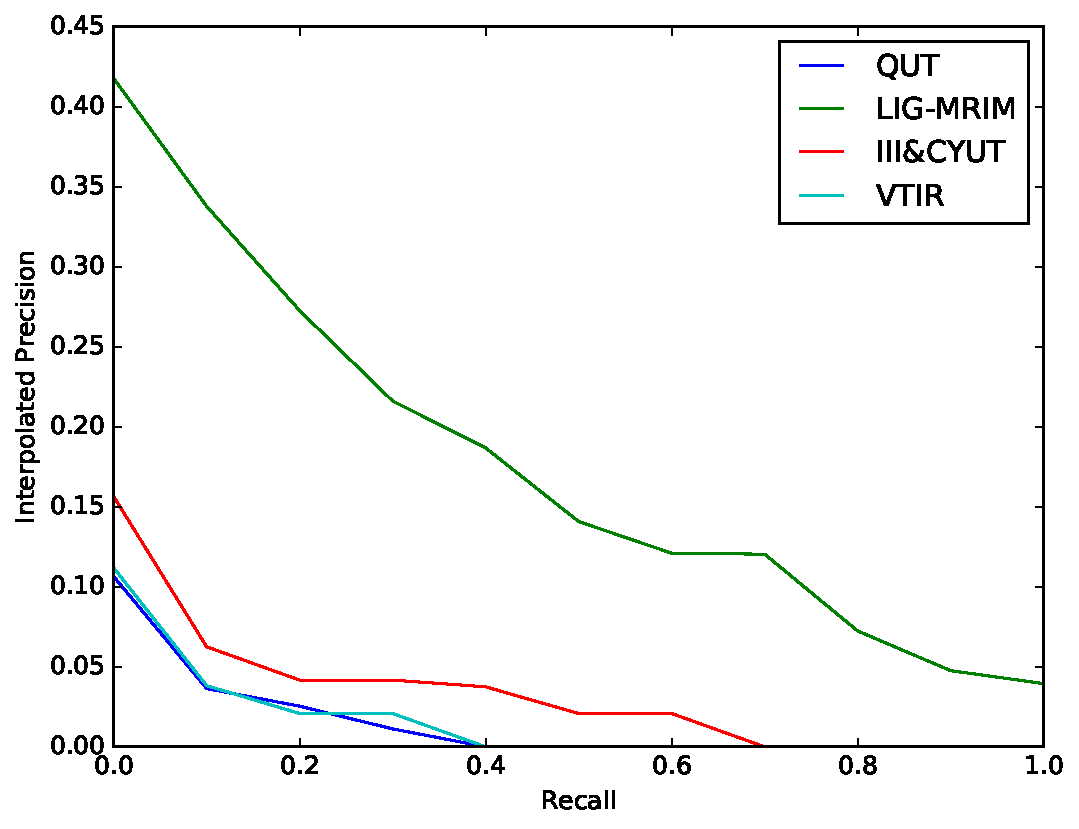
\includegraphics[width=0.95\textwidth]{graphs/ntcir-pr-curve}
    \caption{Precision-recall curves for the four LSAT teams}
    \label{fig:ntcir-results}
\end{figure}
\chapter{Methods}

\section{Sampling Images}

It is not feasible for every image in the NTCIR-12 LSAT data set to be annotated manually. The collection is very large, containing 88,125 images. Moreover it is even more unfeasible to annotate every image four times (for each annotation methodology), thus sampling images to reduce the number of images to annotate is necessary. There are two methodologies employed to sample images: The first builds upon previous work~\cite{scells2016qut} which identifies a way of clustering lifelog images using image histograms for features; and aligning the images temporally to determine cluster segmentation boundaries\footnote{\url{https://github.com/hscells/lifelog-sampling}}. After clustering images, the sampling technique involves selecting one image at random from each cluster. The cosine similarity measure is used to determine if an image should be added to an existing cluster. The threshold value of the cosine between two images is set to 0.86\footnote{This value was empirically found to provide a range of sufficiently different clusters, each containing similar images}. Clusters are then combined based on visual similarity using the aforementioned image histograms and a representative image from each of these clusters is chosen at random. This process results in about 16,000 images for annotation. The second sampling method entails processing the qrels to extract only the relevant images. A maximum of 30 images are selected from each of the 48 topics which results in just over 1,000 images required for annotation. Some topics have less than 30 relevant images which is why the total number of images is lower than what one would expect.

There is some overlap between the images chosen from the clustering process and the images that are known to be relevant, however it overall reduces the number of images to annotate by around 80\%. In reality, it is not expected that all of these images are annotated, rather, the smaller sample set should provide a reasonable interpolation of the larger data set. Annotating both relevant and non-relevant images ensures that retrieval is working correctly: both relevant and non-relevant images should be retrieved, however the images annotated with relevant annotations should rank higher.

The sampled images are uploaded to a database to be annotated. Annotations are then collected through specially designed interfaces.
% Both sampling techniques are required 
% For future work, a combination of clustering and matching images to relevant topics might be a better option, as there will most likely be many irrelevant annotations. There may also be no annotations which are relevant to a topic as well, since the sampling is somewhat random. This makes the process less than idea, but will serve as a proof of concept for further research.

\section{Collecting Annotations}

Once the images have been sampled and uploaded into a database, they are ready to be annotated. Four web interfaces are used to collect of annotations\footnote{\url{https://github.com/hscells/lifelog-ia}}. The interfaces allow experts to annotate images selected randomly from a list of unannotated images. It is important to note that each image is annotated only once and an attempt is made to ensure that there is an overlap between the images and the annotations such that most images annotated should have four annotations.

The architecture of the interfaces consists of:
\begin{enumerate}
    \item A database to store the annotations and the sampled images. The database also records statistical data about each user performing the annotations: who annotated each image, and how long it takes to perform an annotation. This ensures there is a record of who annotated each image, and allows a statistical analysis to be performed at a later stage.
    \item A web server and that handles the `business logic'. This server exposes some password protected RESTful services that applications can hook into.
    \item A website which consumes the API provided by the web server and handles `view logic'. This is the layer that annotators interact with directly. Each interface is one of these views.
\end{enumerate}

The interfaces are designed with great care to ensure collecting annotations is as painless as possible. It is important that the total time it takes to annotate an image (including the time between annotating images, i.e. loading an image) is as small as possible; If it takes a minute to annotate one image, it will take an hour to annotate only 60 images.

% It is for this reason that an automatic captioning system is used to caption the rest of the images. For each methodology, annotations will be generated using a state-of-the-art machine learning architecture. This ensures every single image is annotated, so an annotation has been collected for each image, for each annotation methodology.

\section{Annotation Methodologies}

Four annotation methodologies are selected for investigation: \textbf{textual}, \textbf{tags}, \textbf{relevance assessment} and \textbf{reverse query}. While the annotation types are wildly different to each other, they are all collected in a very similar way. An expert annotator is shown a randomly chosen image from the sampled set of images and is asked to provide an annotation (or in the case of relevance assessment, multiple annotations) for the image. The interfaces used for collecting annotations are pictured and described as follows:

\textbf{Textual}

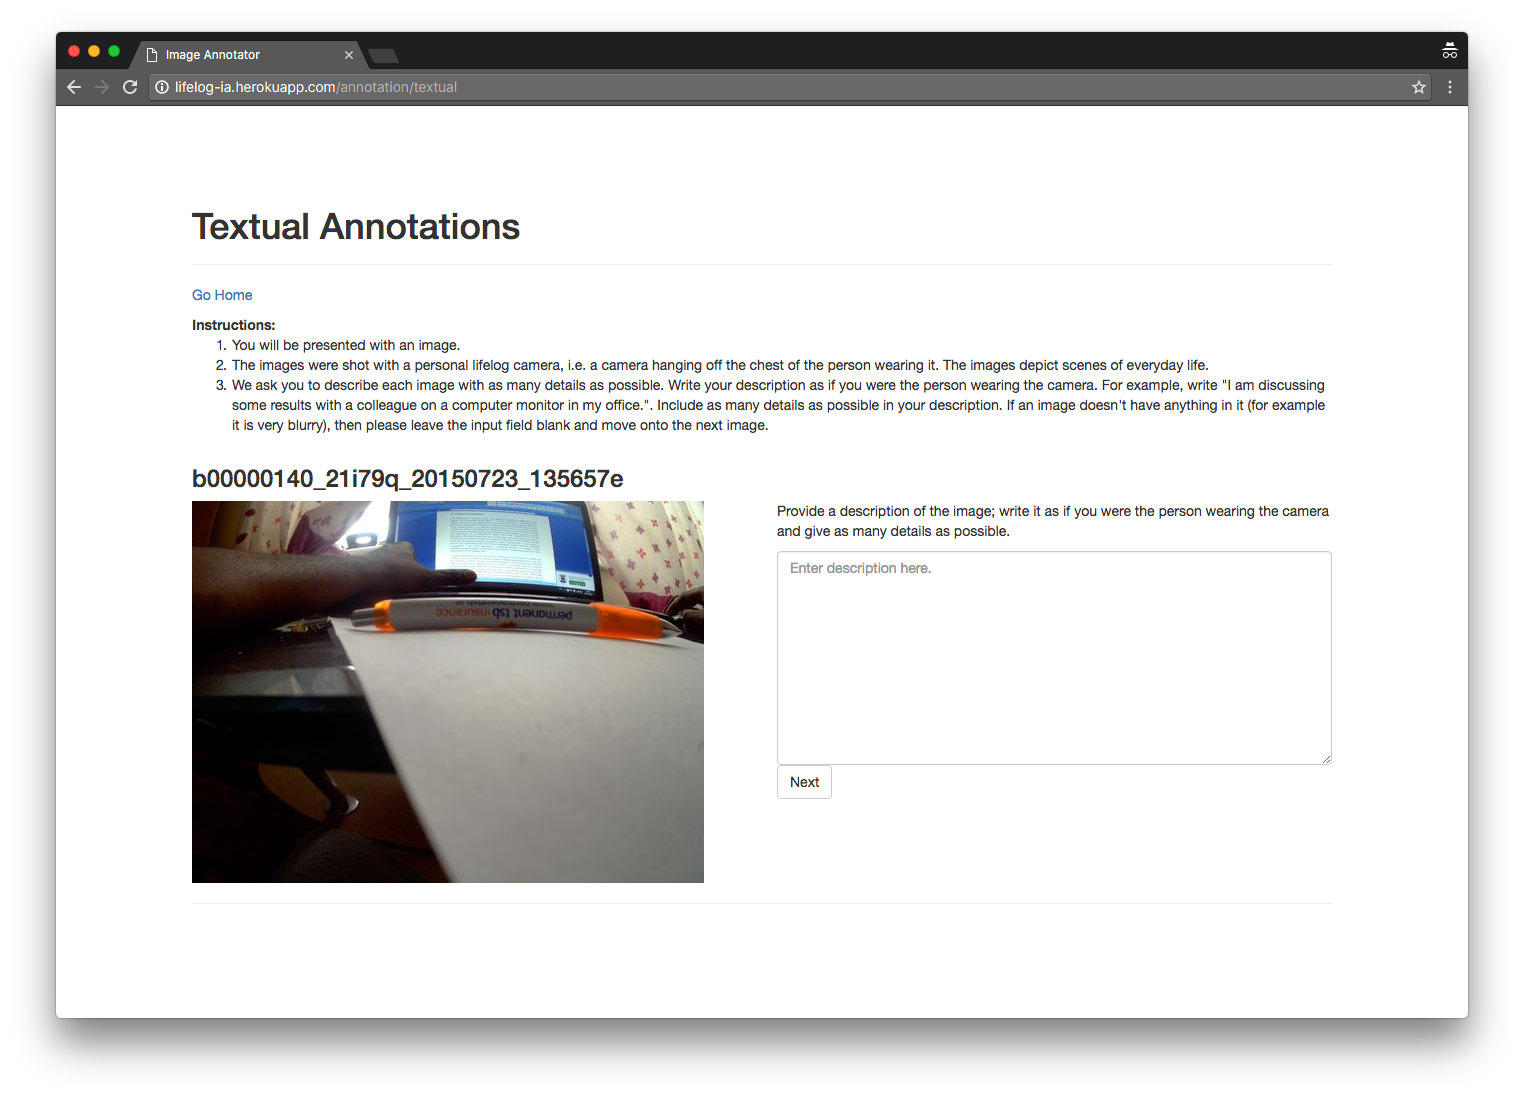
\includegraphics[width=0.95\textwidth]{images/text-interface}

Here, annotations are collected using free form text through a text box on the page. Each textual annotation should contain semantic information about an image, and describe the image with as much detail as possible. These annotations are very similar to a textual document in a typical web search engine, which is why they are selected as one of the methodologies to investigate. Information retrieval is commonly associated with textual documents which contain many sentences with varied semantic and contextual information. This type of annotation highly resembles typical document retrieval and can almost be seen as a baseline, whereas the other annotation methodologies are somewhat novel.

\newpage
\textbf{Tags}

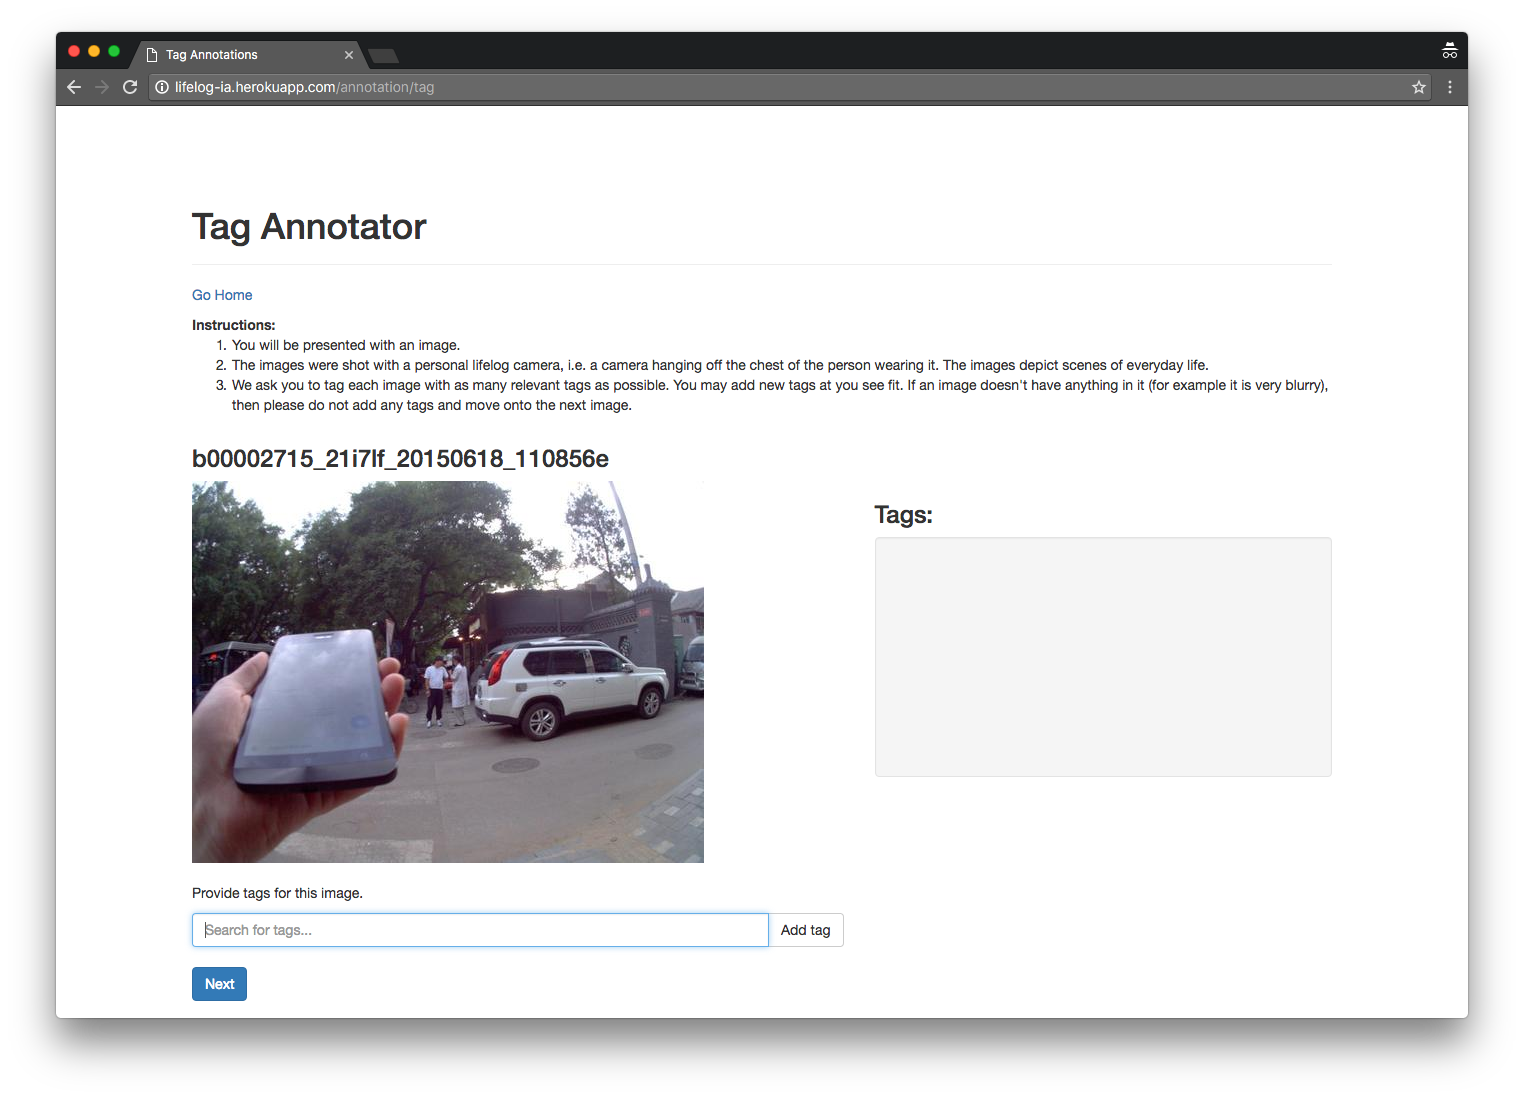
\includegraphics[width=0.95\textwidth]{images/tag-interface}

Tags are collected through this specifically designed interface. The vocabulary of tags is created from previously added tags, the list of tags available is arbitrary and can be expanded. This annotation methodology and style of collection is similar to that seen in other online image tagging scenarios such as Flickr. Similarly, the vocabulary is not restricted to a preset group of terms. This unrestricted vocabulary can result in human error (spelling mistakes), but allows for precise observations about key objects or events in an image. The tags that annotators are allowed to input are allowed to contain more than one word, to cover concepts like `train station' or `shopping mall'.

\newpage
\textbf{Reverse Query}

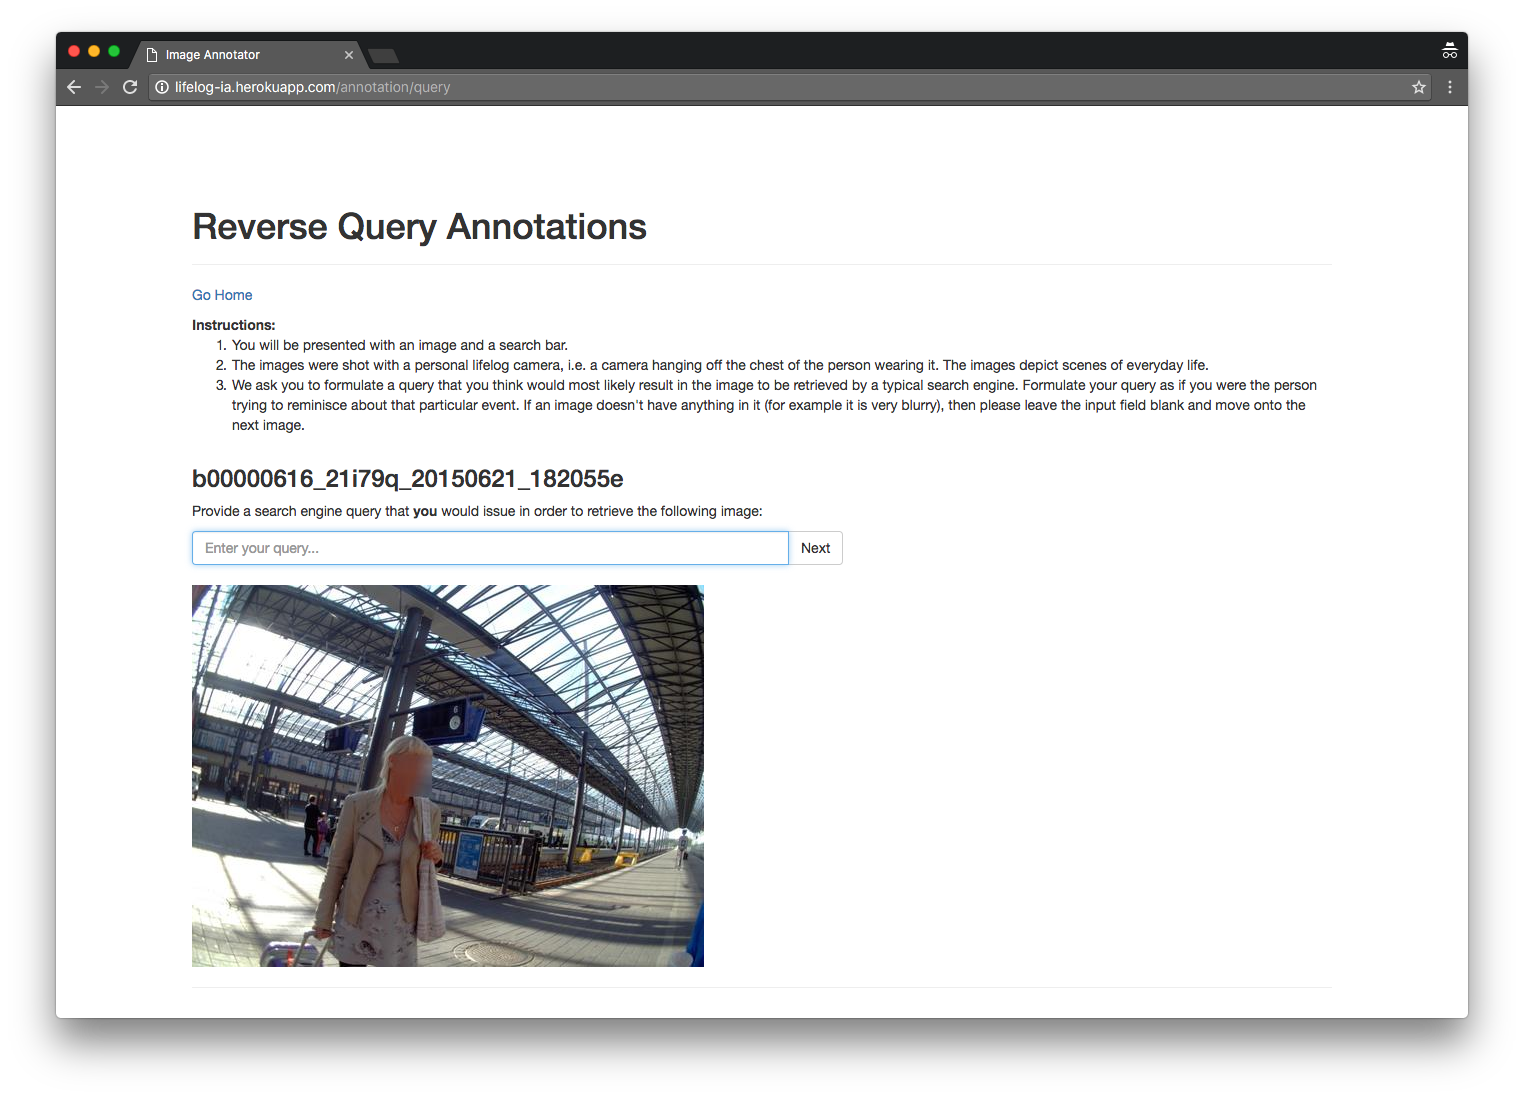
\includegraphics[width=0.95\textwidth]{images/query-interface}

In this interface, user queries are collected by presenting an image taken from the lifelog camera and asking the annotator to provide a query with what they expect to be returned by a typical search engine. This is a relatively novel way of annotating \textit{any} type of document or image~\cite{quteprints82599}. This form of annotation represents the query logs from a search engine. Search engine companies have this data but generally do not make this available due to privacy concerns~\cite{silvestri2010mining}. These annotations are less focused on detail and more focused on one to two key objects or events in the image.

\newpage
\textbf{Relevance Assessment}

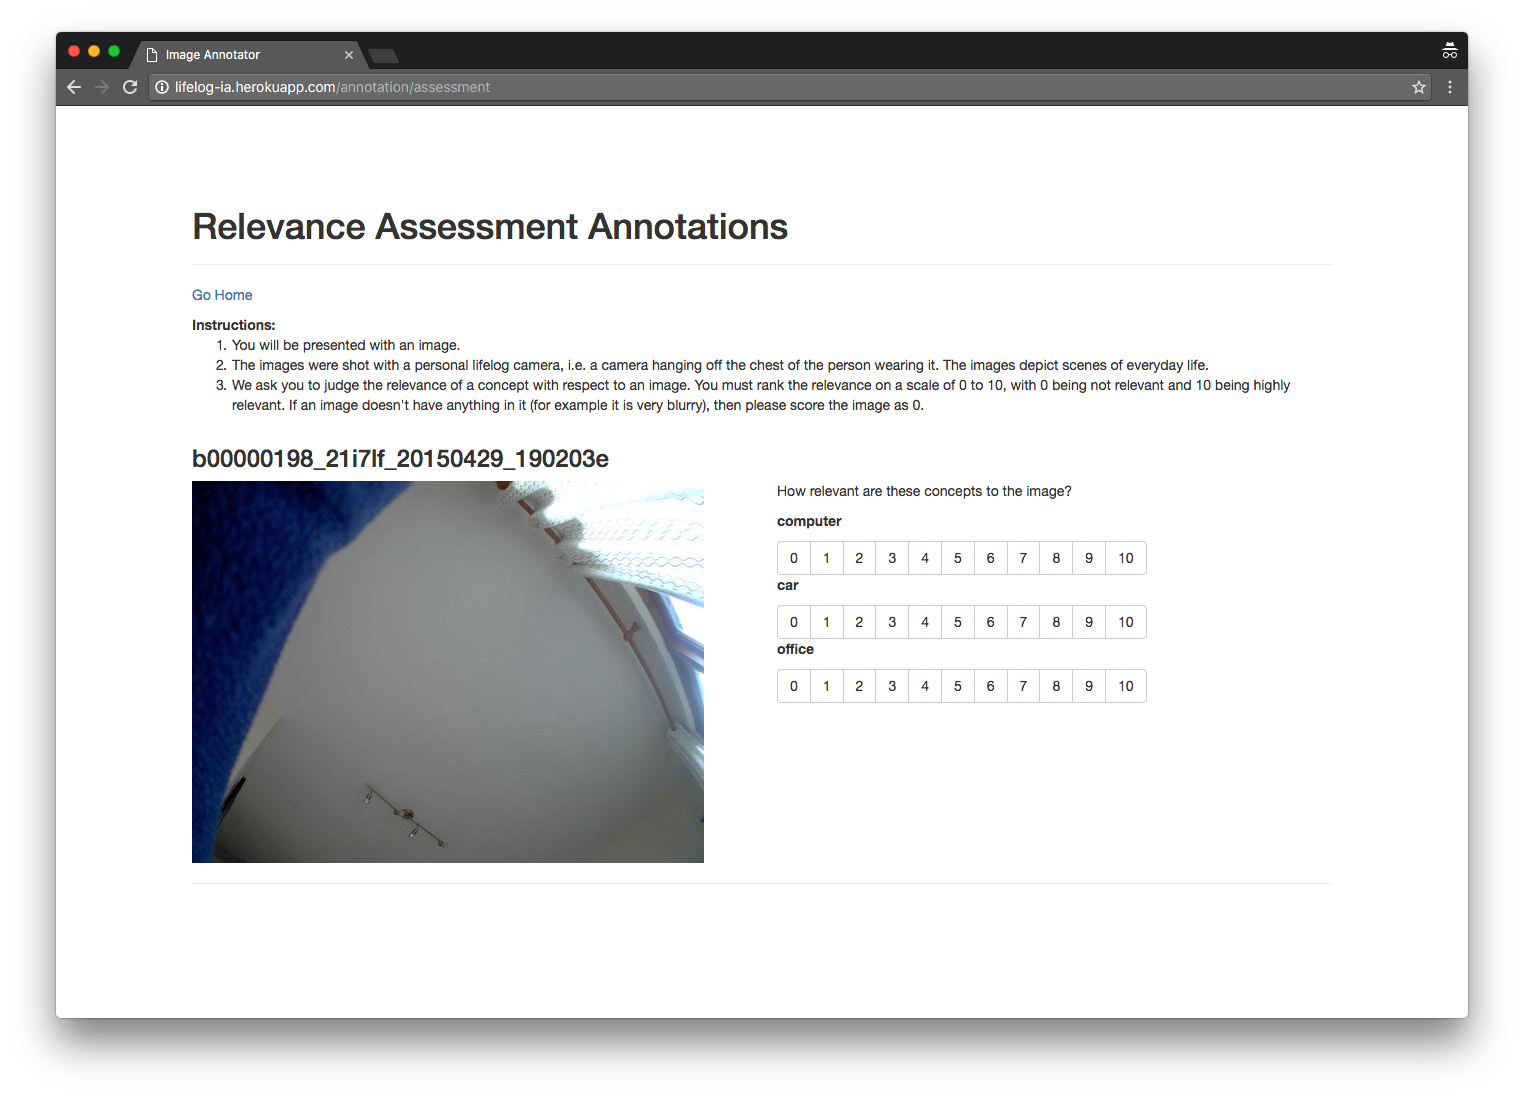
\includegraphics[width=0.95\textwidth]{images/rel-ass-interface}

Relevance assessment involves presenting an annotator with an image, and asking them to judge how relevant a concept is to the image. Assessors are asked to choose concepts from a list to assess, and from those chosen concepts are asked to assess the relevance of that concept to the target image. Concepts are ranked on a scale of zero to ten, where zero is not relevant at all and ten is highly relevant.

These annotations are similar to the tag annotations in that annotators are annotating with some notion of a `concept'. The major difference between the two annotation methodologies is that the vocabulary is finite and the relevance of a concept to the target image is not binary.

Relevance assessment annotations are collected last, the list of concepts is formed from analysing terms in the other annotations. Concepts are chosen by creating a list of terms from the existing textual, tag and query annotations, which are then filtered to the terms that occur in the NTCIR-12 LSAT topic titles and descriptions. Each term is scored using IDF\footnote{Inverse Document Frequency} and then ranked using an algorithm similar to discounted cumulative gain~\cite{jarvelin2002cumulated}; in which higher scoring terms are selected less frequently, and more emphasis is placed on selecting lower scoring terms. 

\newpage
\textbf{Automatic Image Annotation}

Finally, an attempt to automatically caption images for each annotation methodology is done by utilising a recent state-of-the-art machine learning image captioning approach~\cite{karpathy2015deep} which has been open sourced\footnote{\url{https://github.com/karpathy/neuraltalk2}}. The architecture of neuraltalk2 consists of (1) a convolutional neural network (CNN) which learns features of image regions, (2) A recurrent neural network (RNN) that generates textual descriptions using a long short-term memory (LSTM) network. The last layer of the CNN is fed as into into the RNN.

A model is trained in the system described above using the $adam$ optimiser~\cite{kingma2014adam} with $\alpha$ set to 0.8 and $\beta$ set to 0.999. The $adam$ optimiser algorithm is for first-order gradient-based optimisation of stochastic objective functions (i.e convergence in a neural network). The parameters $\alpha$ and $\beta$ represent the step size and exponential decay rates for the moment estimates respectively. The learning rate of the language model is set to 0.0004. Two training attempts are performed: one where the model is trained for a maximum of 70,000 iterations, and another where the model is trained for a maximum of 300,000 iterations. More iterations are performed afterwards to fine tune the deep learning architecture, but in all cases the changes to values of the optimisation function are insignificant.

\section{Evaluating Annotations}\label{methods:evaluating}

Annotations are evaluated with an ad-hoc, TREC style methodology. The topics and qrels from the NTCIR-12 Lifelog semantic access pilot task are used to perform evaluation. In total eight runs are produced: five consisting of each of the manually annotated annotations plus the combination of these, and another four consisting of automatically generated captions for textual, tag, and query annotations as well as the combination of these. This is to investigate if any correlations between the manually annotated annotations and the automatic annotations exist, and to determine if an automatic system can effectively generate suitable annotations for lifelog images. It should be noted that the relevance assessment annotations cannot be learnt by the neural network framework used simply due to the format of the annotations.

Document rankings are generated by submitting queries to ElasticSearch using porter stemmer and a default English stoplist. Queries are formulated by using the title field from the NTCIR-12 Lifelog topics. The stemming and stopping are also applied to the queries. ElasticSearch is also set to only retrieve a maximum of 1,000 images. The runs produced by this system are evaluated using \verb|trec_eval| and the NTCIR-12 Lifelog qrels. The retrieval model for producing runs is $tf*idf$ and the method is the default \verb|simple query string|\footnote{\url{https://www.elastic.co/guide/en/elasticsearch/reference/current/query-dsl-query-string-query.html}} query.

The document rankings and evaluation is performed through a custom-built framework\footnote{\url{https://github.com/hscells/lifelog-eval}}. A Java RESTful application wraps Elasticsearch. This is so a query issued to the Java application can return a properly formatted TREC run, and so many queries can be issued with one request. Rather than the system producing a search listing, it outputs in a format ready for \verb|trec_eval| to process.

\chapter{Results}\label{chapter:results}

The findings of the research is presented in this chapter in the form of the annotation statistics and the retrieval effectiveness of the annotations. The annotation statistics covers the time taken to annotate each annotation methodology, and details about the number of annotations collected. The retrieval effectiveness section provides a breakdown of the performance of both the manually and automatically collected annotations.

\section{Annotation Statistics}

In total, five annotators managed to annotate a total of 10,982 images across all annotation methodologies. These annotators consist of students and staff from an information retrieval group at QUT. Figure \ref{fig:annotator-breakdown} illustrates the number of annotations completed by each annotator. Two annotators account for the majority of the annotations, while three others provide an additional 904. The exact number of each annotation type, the total time it took to annotate each annotation type and the average time it took to annotate is displayed in Table \ref{table:annotation-stats}.

\begin{table}[b]
    \centering
    \begin{tabular}{ | l | l | l | l | p{5cm} |}
    \hline
    Name & Count & Average Time & Total Time \\ \hline
    Text & 3172 & 1 minute & 2 days, 23 hours \\ \hline
    Tag & 2897 & 31 seconds & 23 hours, 40 minutes \\ \hline
    Query & 3616 & 16 seconds & 15 hours, 10 minutes \\ \hline
    Assessment & 1327 & 58 seconds & 21 hours, 36 minutes \\ \hline
    \end{tabular}
    \caption{Annotation statistics obtained by taking the average across all five annotators}
    \label{table:annotation-stats}
\end{table}

\begin{figure}[t]
    \centering
    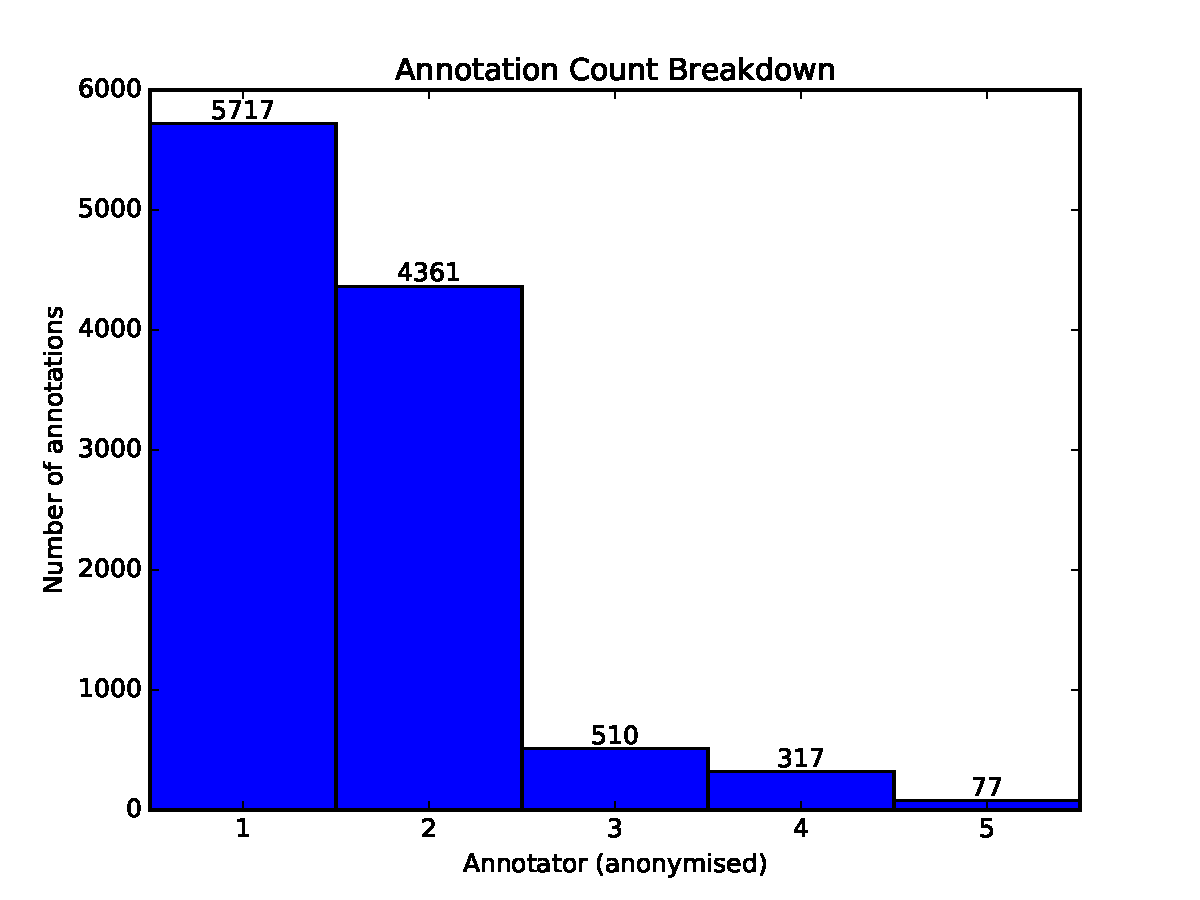
\includegraphics[width=0.8\textwidth]{graphs/annotator-breakdown}
    \caption{Total number of annotations by annotator}
    \label{fig:annotator-breakdown}
\end{figure}

A statistical analysis of the collected annotations reveals that they are appropriate for a typical textual corpus. Figures \ref{fig:idf-scores} and \ref{fig:tf-scores} are what one would expect to see in a Zipfian distribution~\cite{tullo2003modelling}; that is the frequency of each concept is inversely proportional to it's rank in the frequency distribution (the most commonly used concept appears twice as often as the second most frequent concept and three times as often as the third most frequent concept). The notion of concepts are different to terms since a concept can contain more than one word (this is possible through tags, where a tag can contain multiple words such as `shopping mall' and `street sign').

\begin{figure}[b]
    \centering
    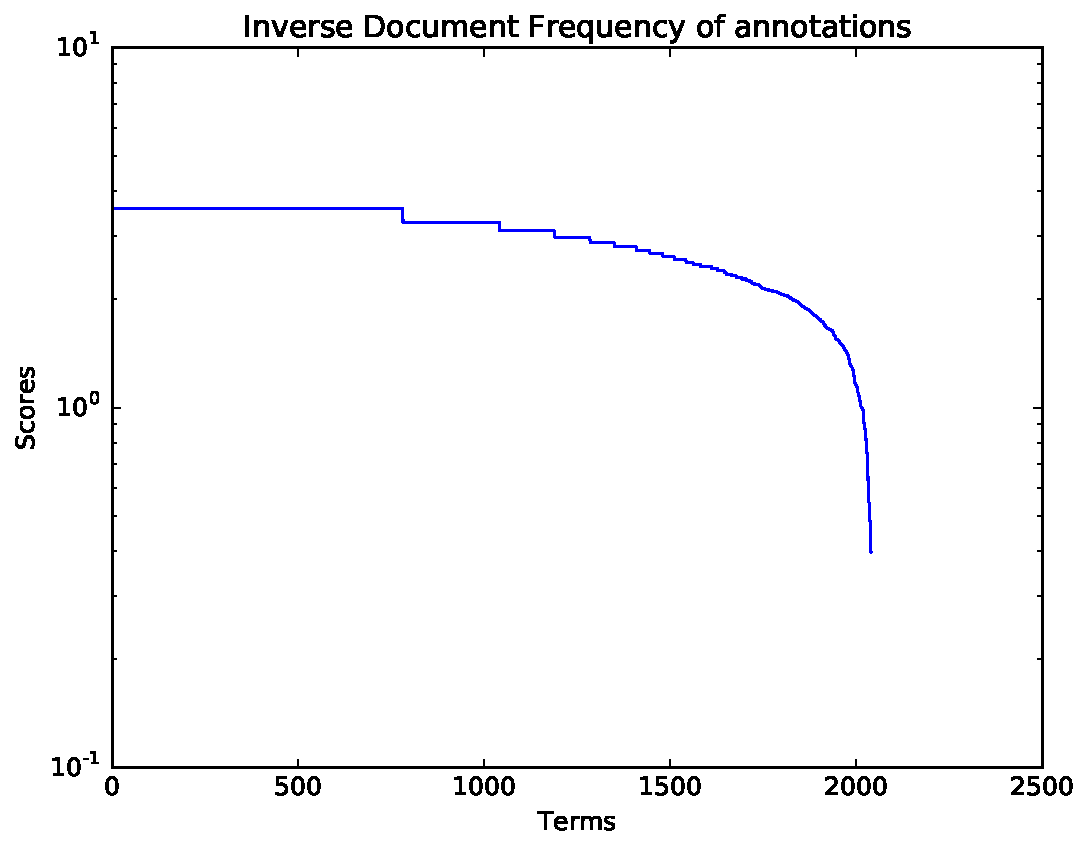
\includegraphics[width=0.7\textwidth]{graphs/idf-scores}
    \caption{IDF scores for concepts in the annotations}
    \label{fig:idf-scores}
\end{figure}

\begin{figure}[b]
    \centering
    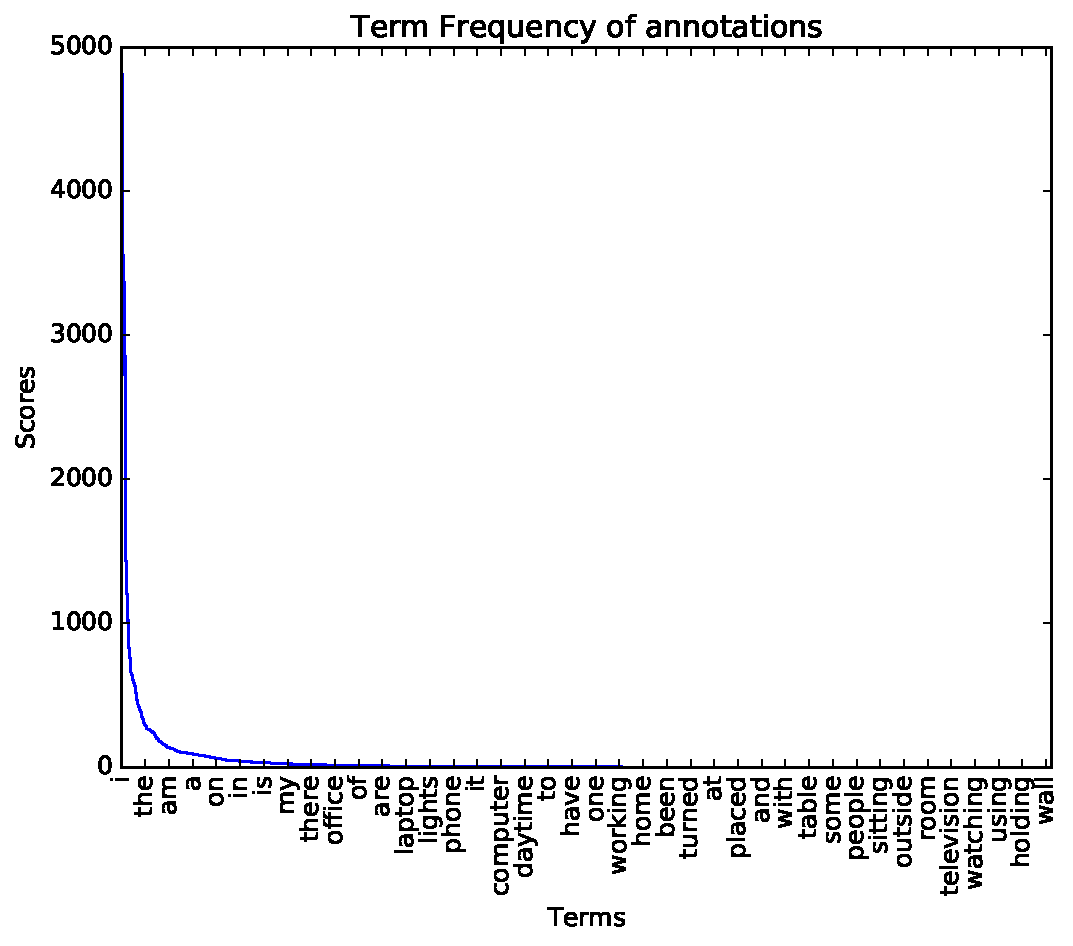
\includegraphics[width=0.7\textwidth]{graphs/tf-scores}
    \caption{Term Frequency scores for concepts in the annotations}
    \label{fig:tf-scores}
\end{figure}

Textual annotations accounted for the highest amount of time taken on average in the collection process. The largest number of annotations collected for a methodology are the query annotations. Qualitative feedback from annotators note that the relevance assessments are the most tedious to collect. Intuitively, formulating a query for a typical search engine does not take a very long time, which can account for the marginal average time for this annotation type. On the other hand, composing (in the annotators mind and physically typing on a keyboard) a descriptive paragraph filled with context and semantics leads to the conclusion that textual annotations do, in fact, take a significant amount of time to annotate. In the same manner, the process of completing a relevance assessment involves scrolling and clicking a multitude of times; this time adds up and is evident in the reported average time.

\FloatBarrier
\section{Retrieval Effectiveness}

Results of each experiment are reported as a table which provides the results from \verb|trec_eval| and as a precision-recall graph. The results from only the manually annotated images are displayed first. Table \ref{table:manual-results} presents the \verb|trec_eval| results for the four annotation methodologies \textit{and} the result of combining all four of the methodologies. The  NTCIR-12 LSAT topics are used for experiments. Among other fields, each topic contains a title and a description; these fields are read as input queries. The title field is more representative of what a typical query looks like when issued by a user. The results of running these experiments are visualised as precision-recall graphs in Figures \ref{fig:manual-result-title} and \ref{fig:manual-result-desc}.

In experiments that use the title field as an input the query annotations perform the best of the four methodologies, however when combining all four collections of annotations together the effectiveness increases slightly, and the precision is higher than the query annotations at high recall (more relevant results). Combining annotations for the experiments that use the description field outperform all four of the methodologies, and the query annotations perform significantly worse.

\begin{table}[ht]
    \begin{tabular}{|c|c|c|c|c|}
        \multicolumn{5}{c}{Topics Titles}\\ \hline
         Methodology & MAP & RR & P@10 & Relevant Retrieved \\ \hline
         Text & 0.3442$^{qc}$ & 0.9223$^{c}$ & 0.8333$^{rc}$ & 1062 \\ \hline
         Tag & 0.5468$^{qcd}$ & 0.9578$^{d}$ & 0.8396$^{rcd}$ & 1040 \\ \hline
         Query & 0.6400$^{tgad}$ & 0.9653$^{rd}$ & 0.8750$^{rd}$ & 1559 \\ \hline
         Relevance Assessment & 0.4815$^{qc}$ & 0.8406$^{qc}$ & 0.6917$^{tgqrd}$ & 831 \\ \hline
         Combined & 0.6495$^{tgrc}$ & 1.000$^{ta}$ & 0.9062$^{tgr}$ & 1612 \\ \hline
         \multicolumn{5}{c}{Topic Descriptions} \\ \hline
         Methodology & MAP & RR & P@10 & Relevant Retrieved \\ \hline
         Text & 0.5285$^{gqc}$ & 0.9792$^{gq}$ & 0.8521$^{gqc}$ & 1088 \\ \hline
         Tag & 0.4627$^{trcd}$ & 0.8928$^{tqcd}$ & 0.7687$^{tqcd}$ & 1055 \\ \hline
         Query & 0.4457$^{tcd}$ & 0.7683$^{tgrcd}$ & 0.5958$^{tgrcd}$ & 1566 \\ \hline
         Relevance Assessment & 0.5219$^{c}$ & 0.9271$^{q}$ & 0.7938$^{tqcd}$ & 972 \\ \hline
         Combined & 0.5855$^{tgqrc}$ & 0.9815$^{gq}$ & 0.8875$^{tgqr}$ & 1613 \\ \hline         
    \end{tabular}
    \caption{MAP, Reciprocal Rank, Precision at 10 scores, and number of relevant retrieved images for the manual annotations. Two tails t-test statistical significance ($p<0.05$) is indicated through the following labels for inter-measurement: text $^t$, tags $^g$, query $^q$, relevance assessment $^r$, combined $^c$. Statistical significance between the same methodology is represented as $^d$.}
    \label{table:manual-results}
\end{table}

\begin{figure}[ht]
    \centering
    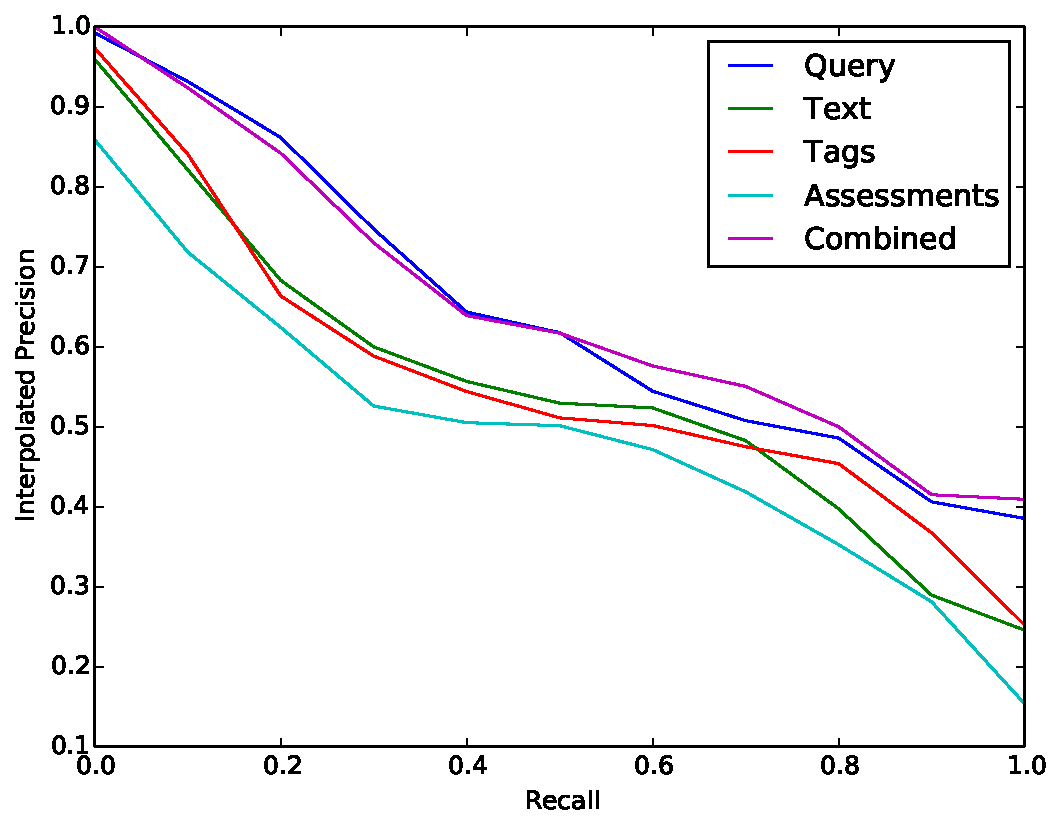
\includegraphics[width=0.8\textwidth]{graphs/manual-title}
    \caption{Precision-recall curves for the manual annotations using topic titles}
    \label{fig:manual-result-title}
\end{figure}

\begin{figure}[ht]
    \centering
    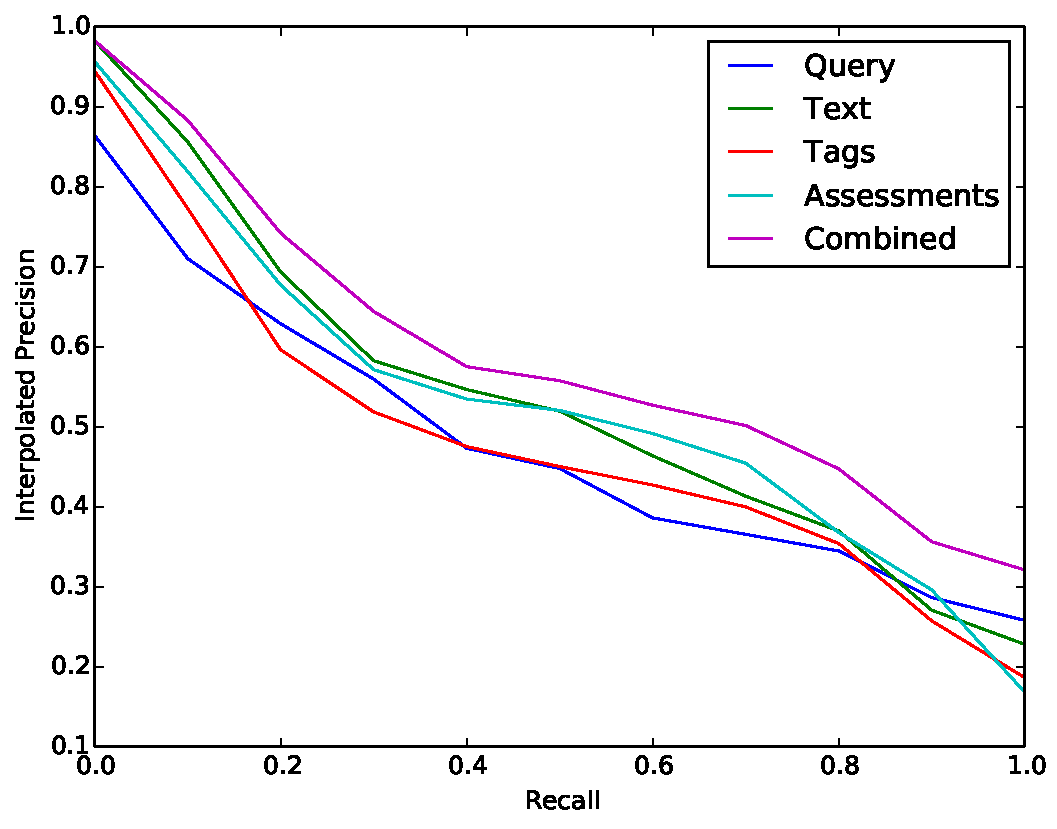
\includegraphics[width=0.8\textwidth]{graphs/manual-desc}
    \caption{Precision-recall curves for the manual annotations using topic descriptions}
    \label{fig:manual-result-desc}
\end{figure}

\FloatBarrier

A neural network framework (neuraltalk2) is trained on the manual textual, tag, and query annotations (i.e. after the manual annotations are collected). Neuraltalk2 is able to produce captions for every image in the collection. The quality of these captions is summarised in Table \ref{table:learnt-results} -- an unfortunate result which could be attributed to the amount of training data. The automatic captions that are generated are evaluated in the same way as the manual annotations. The output of the neural network architecture is formatted to be used in the evaluation pipeline as described in Section \ref{methods:evaluating}. 

There is no clear individual annotation methodology that outperforms the others, the scores are too low to indicate this. Combining the three automatic annotations together does seem to increase the overall precision. The learnt queries do retrieve the most number of images, in a similar result to the manual annotation results.

The number of iterations the neural network architecture covered for each annotation methodology is visualised in Figures \ref{fig:val-loss-1} and \ref{fig:val-loss-2}. The results of the automatic captioning do not get better over time -- in fact they get worse. The gap between topics with a large number of relevant images, topics with a low number of images, and the low number of training examples is presumably the contributing factor to the results in these figures.

\begin{table}[ht]
    \centering
    \begin{tabular}{|c|c|c|c|c|}
        \multicolumn{5}{c}{Topic Titles}\\ \hline
         Methodology & MAP & RR & P@10 & Relevant Retrieved\\ \hline
         Text & 0.0048 & 0.0248 & 0.0196 & 187 \\ \hline
         Tag & 0.0083$^{c}$ & 0.0184 & 0.0022 & 136 \\ \hline
         Query & 0.0076 & 0.0174 & 0.0021 & 246 \\ \hline
         Combined & 0.0164$^{g}$ & 0.0393 & 0.0169 & 337 \\ \hline
        \multicolumn{5}{c}{Topic Descriptions}\\ \hline
         Methodology & MAP & RR & P@10 & Relevant Retrieved\\ \hline
         Text & 0.0048 & 0.0232 & 0.0167 & 222 \\ \hline
         Tag & 0.0050 & 0.0184 & 0.0063 & 145 \\ \hline
         Query & 0.0051 & 0.0062 & 0.0062 & 199 \\ \hline
         Combined & 0.0096 & 0.0470 & 0.0187 & 325 \\ \hline
    \end{tabular}
    \caption{MAP, Reciprocal Rank, Precision at 10 scores, and number of relevant retrieved images for the automatically generated annotations. Two tails t-test statistical significance ($p<0.05$) is indicated through the following labels for inter-measurement: text $^t$, tags $^g$, query $^q$, relevance assessment $^r$, combined $^c$. Statistical significance between the same methodology is represented as $^d$.}
    \label{table:learnt-results}
\end{table}

\begin{figure}[ht]
    \centering
    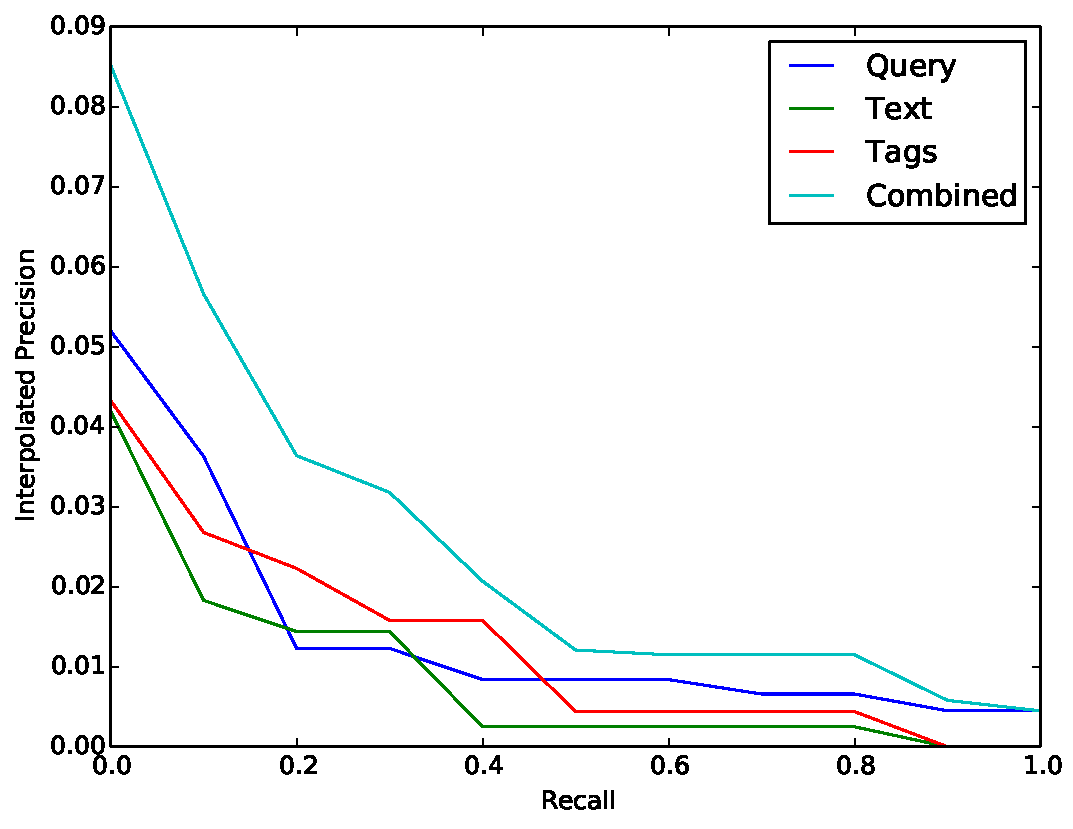
\includegraphics[width=0.8\textwidth]{graphs/auto-title}
    \caption{Precision-recall curves for the learnt annotations using titles}
    \label{fig:auto-result-title}
\end{figure}

\begin{figure}[ht]
    \centering
    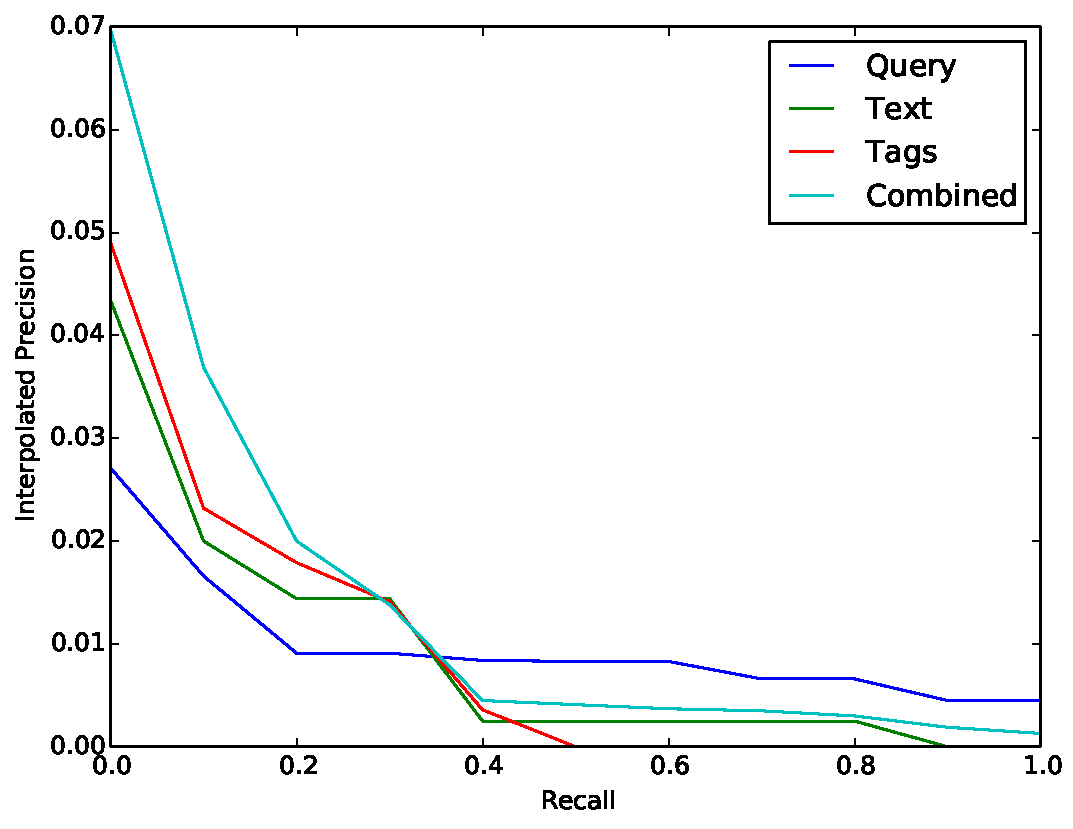
\includegraphics[width=0.8\textwidth]{graphs/auto-desc}
    \caption{Precision-recall curves for the learnt annotations using descriptions}
    \label{fig:auto-result-desc}
\end{figure}

\begin{figure}
    \centering
    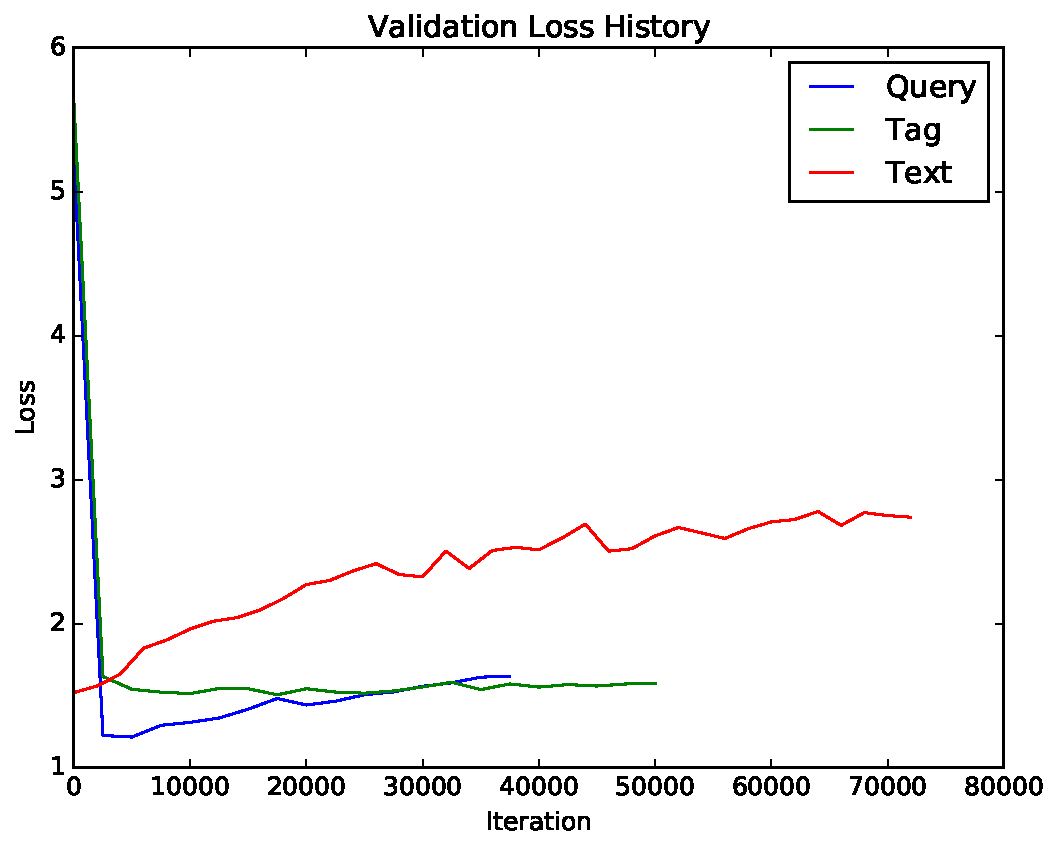
\includegraphics[width=0.7\textwidth]{graphs/initial-validation-loss-history}
    \caption{Validation loss history (\textless 100,000 iterations)}
    \label{fig:val-loss-1}
\end{figure}

\begin{figure}
    \centering
    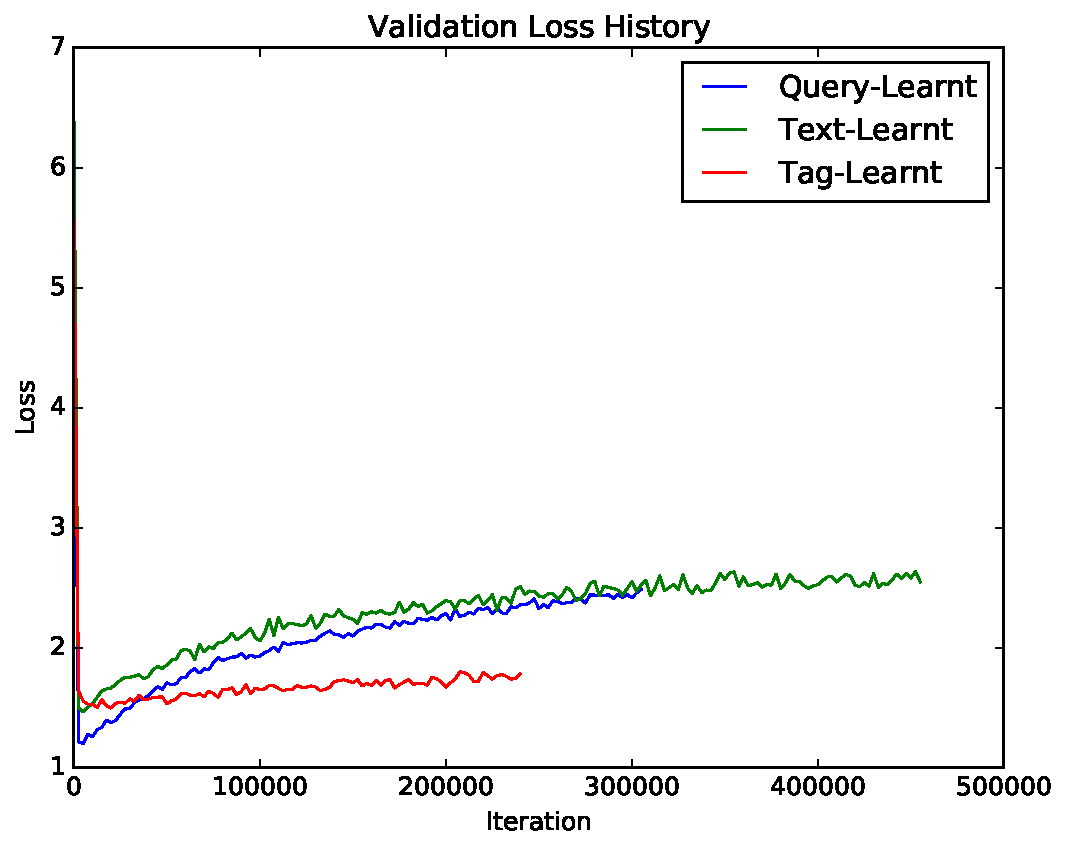
\includegraphics[width=0.7\textwidth]{graphs/validation-loss-history}
    \caption{Validation loss history (\textgreater 200,000 iterations)}
    \label{fig:val-loss-2}
\end{figure}
\chapter{Discussion}

The results from these experiments indicate that of all the types of annotation methodologies, the query annotations provide the best performance also at the lowest cost (i.e the time it took to annotate). It can be seen, however, that by using multiple annotations can increase the interpolated precision as recall approaches 1. It is not surprising to see the tag annotations performing badly, since they simply cannot encode semantic meaning like text and queries, for instance images in the topic `Building a Computer': the term `building' can have more than one meaning, a physical structure and the act of assembling something. The tag annotations did very poorly in this topic, where the textual annotations did the best -- these contain semantics which the search engine can exploit when ranking images.  What is surprising, is that in some situations assessment annotations performed better (however this is most likely due to the fact that there are not many annotations that are not considered relevant). This is most likely do to the fact that the weights of annotated concepts allow the search engine to rank these documents higher. 

In retrospective, the concepts for each query should have been chosen manually based on the topics since some concepts were not present leading to not some topics not having any relevant images. At the time of choosing concepts for use in relevance assessment, there was a large overlap with the titles and the descriptions of the topics and this was seen as good enough. Prior to analysing the results of the relevance assessment annotations, it was thought that they might perform only as well as the images retrieved using tag annotations. Like tags, the concepts of the relevance assessments do not contain semantic meaning; however unlike tags, each concept is assigned a weighting of how relevant it is to an image. In assigning weights, the concepts assigned to images are contextualised; now `building' is highly relevant \textbf{and} `computer' is highly relevant, as opposed to another image that may have an equally high weight for `building' but a high weight for `architecture'. The image with the high `computer' concept will be ranked higher because of the weighting; this explains why relevance assessments outperforms the tagging approach even though less topics were retrieved. The trade-off in the end is that tagging takes half as long for the same if not worse retrieval performance.

The topics themselves it seems were not originally intended to have individual images annotated. Relevant images in a topic are actually a group of images or a `moment'. Each topic has several relevant moments, of which some contain images that do not seem to be relevant to the topic at all. As a general rule these images that did not look relevant, even though they were considered to be by the task organisers were not annotated as relevant. For instance, in the topic `Conversation while eating', the lifelogger often wipes his mouth with a serviette blocking the camera. Images such as these were not assigned any annotation. Grouping images into moments may have also sped up the annotation process; annotating several images considered to be a moment might not only have made collecting annotations less tedious and time consuming, but could also have allowed for more images to be annotated. The downside to this however may have been that these irrelevant images crop up inside each moment. One way to avoid a situation like this would be to let the annotator simply remove any images which are covered by objects or too blurry to make anything out.

\begin{figure}[h]
    \centering
    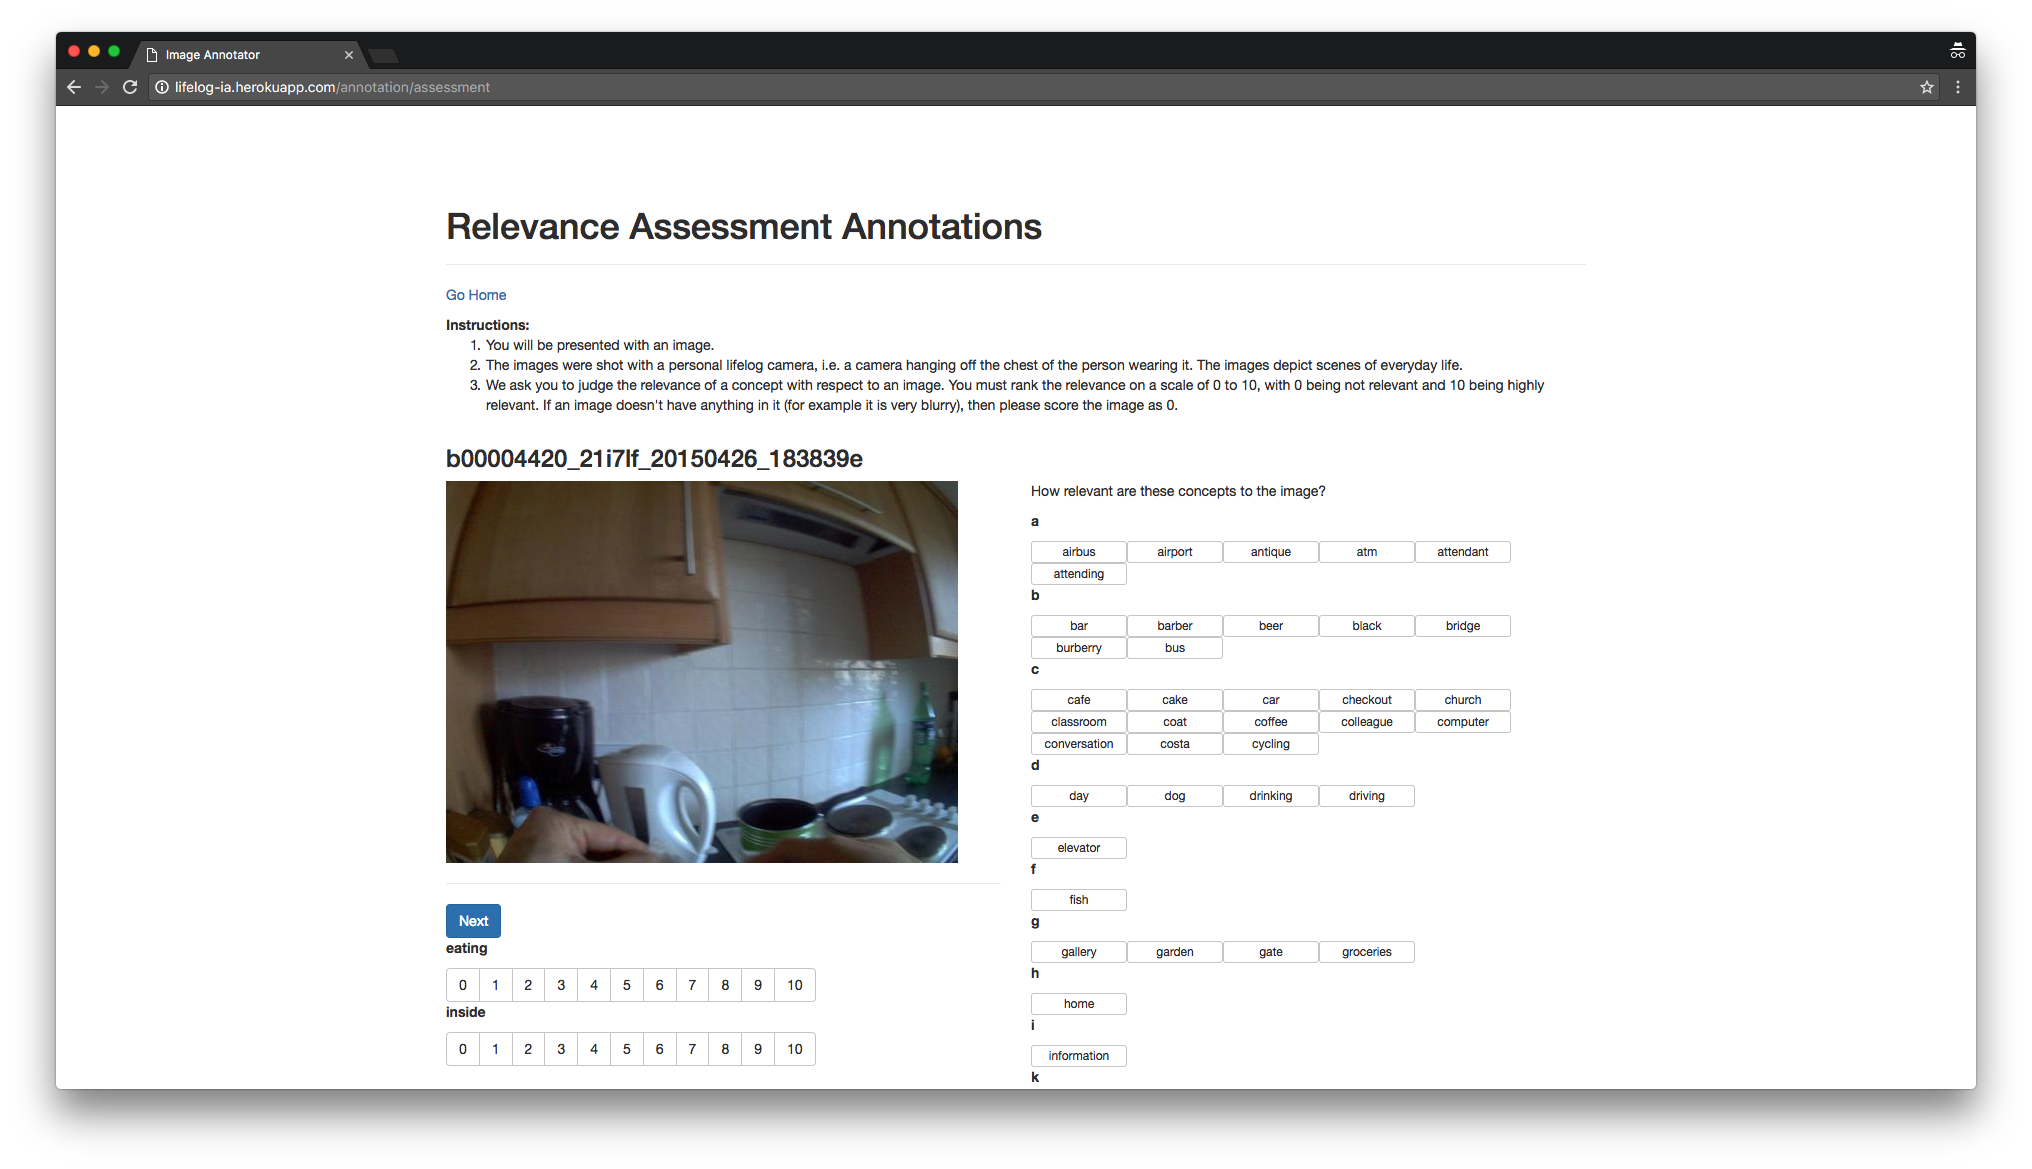
\includegraphics[width=0.95\textwidth]{images/new-rel-ass-interface}
    \caption{Updated query annotation interface}
    \label{fig:new-rel-ass}
\end{figure}

The interfaces themselves also went through many changes, both big and small. The biggest change from the initial design was for the relevance assessment interface as seen in Figure \ref{fig:new-rel-ass}. Here, each concept is grouped alphabetically; when one is clicked, assessments are added underneath the image. Here not every caption must be assessed manually. When the next button is clicked, all unassessed captions are automatically considered not relevant.

In total, there are only 6,657 images which the NTCIR-12 LSAT organisers considered to be relevant; from a collection of 88,125 images in total (only 7.5\%). If images were only annotated from the clustering method of sampling images, only 16,014 images (18\% of the data set) could be annotated. Of that, 1,176 images are considered relevant. This is why the second method of sampling images is so important -- the clusters do not provide a good distribution of relevant and non-relevant images to annotate if we just pick at random.


% - While there is an overlap of the terms in the annotations and queries, this does not necessarily mean that the terms in the annotations are used within the same context. This is particularly evident in the tag annotations. The term `key' is relevant to a query where the person wearing a lifelog camera is getting a key replaced, but the term was also found within the context of someone using a `key card' to enter their office.

% The topics were not designed to have images annotated individually out of order. Topics were designed with a range of images that are relevant, or a `moment' of images. 

% - even though images are chosen from random from a smaller pool of images, it simply was not enough to pick at random. The qrels identified 6657 images that should be relevant. From here, the pool of sampled images only contains 1179 images. Only 17.7\% of the images in the images chosen by clustering can be annotated.

The selection of image to be annotated also intuitively must impact the way a neural network captions images. If a topic contains a diverse range of locations and actions but the images sampled for annotation only cover one of these locations then it seems obvious that many images will get miscaptioned. In hindsight, taking the time to select a variety of perspectives and locations within a moment to cover edge cases might have increased the accuracy of the captions; but it is unclear by how much. It could also be the number of training examples required --- there simply may not have been enough annotations for the neural network to learn (a terrifying thought). One thing that can be said for certain is that the number of training iterations required is not the limiting factor in generating accurate captions. Over 200,000 iterations were performed for the three methodologies, and all of them got worse over time. An acceptable number of iterations for this particular setup appears to fall between 30,000 and 100,000; depending on the type of annotation.


% differences between each annotation methodology - All of them are very different to each other, which presents some interesting problems such as how long it takes to annotate each image, how can each annotation methodology be evaluated etc


% text
% Textual annotation are the most time consuming annotation type to collect. Many images contain two or more highly relevant events or `important' objects. Describing these can take annotators up to several minutes each. This is opposed to all the other annotation methodologies where most images can be annotated in a minute or less.

% tags
% In terms of evaluation, tags may be the opposite of textual annotations; intuitively tags should be the best at training an image classifier and are expected to perform the worst when embedded a search task. Tags, however, may be very good at boosting the performance of other annotation types in the search task when combined. For instance, searching on the text \textit{and} tags fields may increase the scores of text annotation alone.

% query
% and therefore it is unknown how well the collected queries will perform in search or for training an image classifier. The level of detail in these annotations will be very low, since most queries should be short in length.
% Much like tags, this annotation type will be very easy to collect. Formulating a query for an image should not takz a significant amount of time. There is the problem of bias \todo{Is there really? I should investigate this further}
\chapter{Conclusions}

\section{Contribution Summaries}

\textbf{How can annotations for a collection of lifelog images be evaluated?}

\textbf{What are the possible ways lifelog images can be annotated and what is their retrieval effectiveness?
}

\textbf{How do annotations generated by current state-of-the-art automatic image captioning techniques compare to the effectiveness of manual annotations?}


\section{Future Work}

\textbf{Image Interfaces}

The most important change to make if continuing this research is to segment the collection of images into moments rather than individual images. This would allow many more images to be annotated in a smaller amount of time and cover more edge cases. New techniques are required to sample images into moments rather than individually, and the image annotation interfaces must be updated to reflect this. 

Adding and removing images from each moment in the annotation interfaces is necessary (the sampling process is not likely to perfectly capture all relevant images in a moment i.e there could be outliers on the edges of the moment). One thing that needs further investigation is whether to overlap moments with each other. Is it sensible to annotate images more than once if they appear in moments which overlap?

\textbf{Automatic Captioning}

Automatic captioning tools seem to work very well in other domains and it is unfortunate that this research could not exploit them. The number of annotations used as training data is the most likely reason this research could not generate captions effectively. Although diverse in moments and objects, there are still less than 100,000 images in total, with less than 20,000 of these images considered `relevant'. Many topics have less than 100 relevant images so using a data set with more relevant images may improve how images get captioned. 

The retrieval system itself can also be expanded up to combine TBIR and CBIR systems. There has been recent work done to generate images from textual descriptions by Reed et. al~\cite{reed2016generative}; however it looks limited to small categories and the resolution of the generated images are low. It is not difficult to imagine a system which generates images from a query and retrieves using an image similarity technique. As of writing this, the idea is only a pipe dream; the future of automatic captioning and image retrieval of lifelogs is bright.

\textbf{Image sampling}

Given more time, it would be worthwhile investigating other image similarity measures (such as those used by the LEMoRe team ~\cite{de40lemore} at NTCIR-12) to possibly produce a more uniformly distributed sample set.

% There has been some work on generating images based on textual descriptions, but it looks limited to small collections of images, and does not seem to be able to produce large resolution images. In the future, search may be able to be performed by image description->image generation->image matching \todo{this https://github.com/paarthneekhara/text-to-image and the paper should be cited here}
 
% Current state of the art automatic image captioning algorithms~\cite{karpathy2015deep} allow many images to be textually annotated with some level of accuracy. 
 
% The collection of images used is still relatively small. Although diverse in moments and objects, there are still less than 100k images. A large-scale test collection in the magnitude of hundreds of thousands of images to a million or more images could offer better results. \todo{I have read some discussions on line about this but I am yet to find any papers/formal research on this, as well as the exact number of images}. Results will only get more accurate because there is a more diverse range of events happening in the collection.

% There are four annotation types under investigation. Each one is very different to the last. There have been no studies into the most effective methodology or set of methodologies for annotating lifelog images. It would be nice to investigate more than four, however due to time constraints this is inconceivable.

% \begin{appendices}
% \renewcommand\thetable{\thesection\arabic{table}}
% \renewcommand\thefigure{\thesection\arabic{figure}}
% \section{Format of Collection} \label{app:format}
% \end{appendices}

\bibliographystyle{abbrv}
\bibliography{thesis}

\end{document}
